\chapter{Análisis y estudio de los métodos de PE propuestos}

Una vez expuestas todas las condiciones del entrenamiento, como los modelos a probar, las métricas, funciones de pérdida y presentados los datos, podemos dar paso al entrenamiento. Sin lugar a dudas, es la fase más lenta de todo el proceso, la cual ha prolongado su desarrollo considerablemente. El objetivo es claro: poner a prueba las 5 propuestas realizadas para establecer, en primer lugar, cuál o cuáles de ellas son competitivas, y posteriormente, evaluar cada encoding sobre todos los conjuntos de datos para medir la ganancia con respecto a la propuesta original formulada por Informer~\cite{zhou2021informerefficienttransformerlong}.


\section{Experimentación previa. Elección del tamaño de ventana}

Antes de comenzar con la comparativa de los encodings formulados, debemos tener en cuenta un parámetro clave en el rendimiento: ¿Qué tamaño de ventana es el adecuado?.\\

Este valor es un parámetro de entrada común a las cinco variantes de encodings propuestas en este trabajo, y determina cuánta información del entorno se toma como parte del contexto de cada posición, enriqueciéndolo con información asociada a estadísticas y los rezagos anteriores. Un tamaño de ventana excesivamente grande puede provocar que los valores estadísticos sean demasiado genéricos, y no aporten información útil al mecanismo de atención, mientras que una ventana demasiado pequeña puede contener demasiado ruido, y no sea útil para el modelo, e incluso, dificulte la detección de patrones.\\

Por tanto, lo ideal es emplear algún método de búsqueda de parámetros que nos permita probar con diferentes configuraciones y escoger la que mejor resultado ofrezca. Pero en conjuntos de datos de gran tamaño, esa tarea es prácticamente imposible debido al tiempo que sería necesario para realizar cada prueba. Por tanto, para disponer de una heurística a seguir, y que sea estimable en un tiempo reducido, podemos tomar las variantes horarias del dataset ETT, de tamaño reducido, y realizar un pequeño experimento: tomar los valores de longitud de secuencia, etiqueta y predicción empleados en el paper original de Informer y probar con diferentes tamaños de ventana entre 3 y longitud de secuencia.\\

Estos parámetros son:

\begin{itemize}
	\item Longitud de secuencia: 96
	\item Longitud de etiqueta: 48
	\item Longitud de predicción: 24
\end{itemize}

Para realizar el estudio de forma intuitiva y visual, hemos recopilado los resultados del análisis de forma gráfica: se han ejecutado ETTh1 y ETTh2 con todos los valores de ventana entre 3 y 96, y ejecutado cada configuración 10 veces para obtener así un valor promedio estable, pues al evaluar tamaños de ventana muy juntos las diferencias serán mínimas y así reducimos el efecto del ruido sobre el MSE todo lo posible. Los resultados los podemos encontrar en las figuras \ref{mean_mse_vs_window_ETTh1} para ETTh1 y en la \ref{mean_mse_vs_window_ETTh2} para ETTh2, marcando en negrita los 5 mejores resultados obtenidos.\\


\begin{figure}[H]
	\centering
	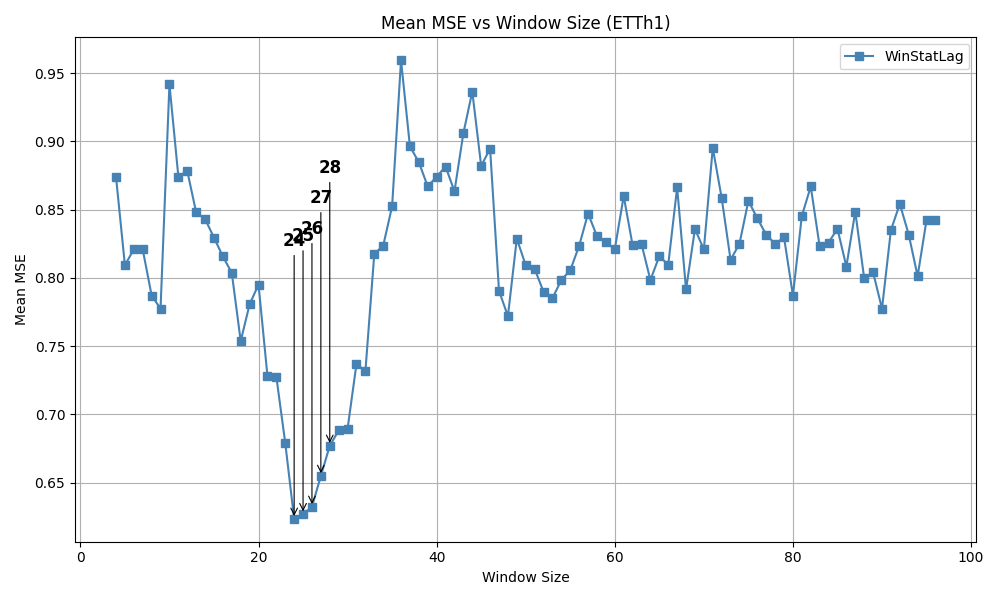
\includegraphics[scale=0.475]{img/mean_mse_vs_window_ETTh1}
	\caption{Estudio del tamaño de ventana mediante MSE (ETTh1)}
	\label{mean_mse_vs_window_ETTh1}
\end{figure}


\begin{figure}[H]
	\centering
	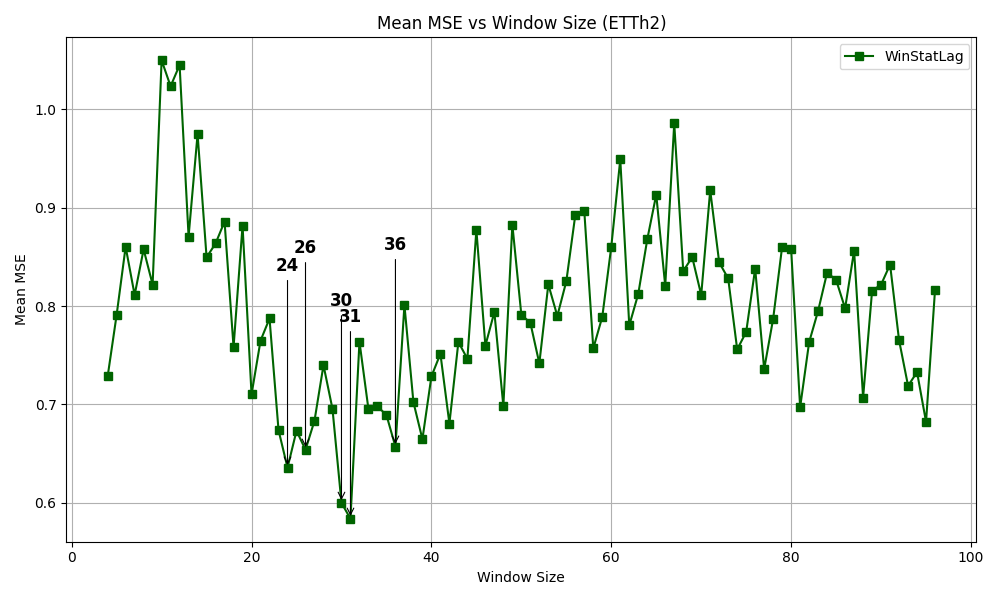
\includegraphics[scale=0.475]{img/mean_mse_vs_window_ETTh2}
	\caption{Estudio del tamaño de ventana mediante MSE (ETTh2)}
	\label{mean_mse_vs_window_ETTh2}
\end{figure}

En ambos casos, los valores se sitúan entre el 24 y el 36, siendo el 24 exactamente $1/4$ del valor de longitud de secuencia, 96, y el 36 algo más de la tercera parte de este. Por tanto, una heurística razonable podría ser ubicar el valor de tamaño de ventana entre una cuarta o tercera parte de la longitud de secuencia. Si bien deducir este resultado tan solo de dos conjuntos de datos puede ser demasiado optimista, al menos nos permite tener un punto de partida, sabiendo que en el resto de conjuntos sería imposible realizar un experimento de este tipo en un tiempo razonable.\\

\section{Análisis experimental de los encodings propuestos}

Una vez justificados los procedimientos de comparación, y determinada la heurística para el tamaño de ventana, podemos comenzar a analizar los resultados obtenidos en el entrenamiento de cada propuesta. \\

La estructura seguida por los experimentos será la siguiente: primero, evaluaremos cuales de las cinco propuestas formuladas obtiene el mejor rendimiento sobre un conjunto de referencia, Household Power Consumption~\cite{hebrail2006individual}, para así descartar potenciales alternativas pobres, y posteriormente, procederemos a analizar su utilidad en el resto de conjuntos de datos.\\

\subsection{HPC: Evaluación de PE}

El dataset de Individual Household Power Consumption ha sido el conjunto escogido para discriminar en un primer instante los mejores métodos de los cinco propuestos. Esta decisión viene motivada por dos aspectos; en primer lugar, este conjunto de datos dispone de una longitud suficiente para inferir la información relevante de la serie y realizar predicciones a largo plazo, y además, en el comportamiento de sus variables vimos aspectos como la estacionalidad, la cual es más difícil de modelar para un Transformer, pero también la ausencia de estacionalidad en ciertas variables, lo cual ha sido tradicionalmente un problema para la aplicación de métodos clásicos.\\

No obstante, la decisión de escoger un dataset únicamente para esta tarea viene motivada por el coste computacional: evaluar todas las alternativas en cada uno de los conjuntos de datos podría requerir semanas e incluso meses para completar por cada dataset, lo cual se escapa de los recursos y limitaciones temporales de las que disponemos.

\subsubsection{Análisis y resultados}

Escoger un conjunto de datos como este, de aproximadamente 2 millones de mediciones, y 7 características, supone un interesante campo de pruebas para las codificaciones. Para la comparativa, realizaremos las siguientes ejecuciones:

\begin{itemize}
	\item Informer con configuración por defecto.
	\item PE sinusoidal.
	\item Nuevas propuestas: WinStat, WinStatLag, WinStatFlex,  WinStatTPE y WinStatSPE	
	\item Sin PE.
\end{itemize}

Para realizar una comparativa justa de los resultados, se han empleado en todos los casos los mismos parámetros, de forma que criterios como la longitud de secuencia, la longitud de contexto o la longitud de predicción no afecten a los resultados. La arquitectura y los parámetros asociados se pueden ver en la tabla \ref{ajustes}.

\begin{table}[!ht]
	\centering
	\begin{tabular}{l|l}
		\toprule
		Parámetro & Valor \\
		\midrule
		{Modelo de atención} & Vanilla \\
		{Tamaño de batch} & 32 \\
		{Dropout} & 0.2 \\
		{Nº de ejecuciones} & 3 \\
		{Tamaño de ventana} & 60 \\
		{Longitud de secuencia} & 180 \\
		{Longitud de etiqueta/contexto} & 60 \\
		{Longitud de predicción} & 60 \\
		\bottomrule
	\end{tabular}
\caption{HPC: configuración de parámetros comunes empleada para los experimentos}
\label{ajustes}
\end{table}

\paragraph{Informer}

En primer lugar, comenzaremos por ejecutar el modelo original de Informer. De esta forma, tendremos una referencia de partida que nos sirva para comparar las propuestas siguientes, y ver si están siendo efectivas. Por defecto, Informer usa codificación de tipo seno-coseno, pero adicionalmente, incorpora información de los timestamps a través de un mecanismo llamado timeF. Son características adicionales que tratan de ayudar al modelo a capturar patrones periódicos y estacionales en la serie temporal, aunque de manera bastante limitada. 

\begin{table}[!ht]
	\centering
	\begin{tabular}{l|N|N}
	\toprule
	\text{Métrica} & \text{Media} & \text{STD} \\
	\midrule
	MSE & 0,532965 & 0,010976 \\
	MAE & 0,415272 & 0,012216 \\
	MAPE & 2,598725 & 0,066858 \\
	MSPE & 1345,903158 & 113,73071 \\
	RMSE & 0,730005 & 0,00754 \\
	TrainTime(s) & 7817,02026 & 821,270911 \\
	TestTime(s) & 91,941244 & 1,244423 \\
	\bottomrule
\end{tabular}
\caption{HPC: resultados para Informer}
\label{hpcinf}
\end{table}

Los resultados de la ejecución pueden apreciarse en la tabla \ref{hpcinf}. En ella, podemos notar que la varianza en los resultados, tras ejecutar 3 iteraciones, es bastante pequeña, e inferior a la centésima tanto para MAE como MSE. Sin embargo, las tasas de error en las métricas de MAPE y MSPE se disparan: esto se debe a su gran sensibilidad a valores pequeños, ya que todas las mediciones han sido normalizadas, por lo que no deberían ser consideradas como una forma de comparación debida su inestabilidad. En el caso de RMSE, el error también es bastante alto, de un 73\%, fruto de la misma debilidad que la mostrada en MAPE y MSPE.\\

En términos de eficiencia computacional, podemos utilizar el tiempo medio de ejecución como referencia. En promedio, una ejecución del modelo por defecto requiere aproximadamente 7817 segundos, equivalentes a casi 2,17 horas. Aunque este tiempo resulta razonable considerando la longitud del conjunto de datos, su utilidad real es servir como valor de referencia para evaluar el coste adicional que implican las operaciones introducidas en los modelos alternativos que veremos a continuación.

\paragraph{PE sinusoidal}

Continuando con el modelo de referencia, daremos un segundo paso. Teniendo en cuenta el impacto limitado de la información añadida por timeF, ¿es realmente relevante frente a la información proporcionada por el encoding de tipo seno-coseno?. Para conocerlo, hemos realizado una ejecución suprimiendo esta componente, convirtiendo la arquitectura en prácticamente la definición de un Transformer vanilla para procesamiento de lenguaje.\\

Sorprendentemente, los resultados obtenidos, visibles en la tabla \ref{hpcfixed} son muy similares a los vistos en el modelo original: la pérdida de rendimiento en métricas es prácticamente despreciable, con una diferencia de rendimiento inferior a la centésima para el MSE (0,5329 vs 0,5377) y un caso similar en MAE (0,4152 vs 0,414), obteniendo incluso un mejor el resultado para esta codificación. Esto nos indica que la información adicional aportada en el modelo original no estaba aumentando considerablemente el rendimiento del modelo.\\

\begin{table}[!ht]
	\centering
	\begin{tabular}{l|N|N}
	\toprule
	\text{Métrica} & \text{Media} & \text{STD} \\
	\midrule
		MSE & 0,537721 & 0,011375 \\
		MAE & 0,414084 & 0,006756 \\
		MAPE & 2,573043 & 0,094281 \\
		MSPE & 1363,108439 & 117,15614 \\
		RMSE & 0,733254 & 0,007743 \\
		TrainTime(s) & 10741,03553 & 422,837205 \\
		TestTime(s) & 225,145923 & 63,83665 \\
		\bottomrule
	\end{tabular}
	\caption{HPC: resultados para encoding seno-coseno}
	\label{hpcfixed}
\end{table}


Sin embargo, resulta relevante destacar que el tiempo de ejecución aumenta significativamente, alcanzando aproximadamente 10741 segundos (cerca de 3 horas) en el entrenamiento. Aunque este resultado pueda parecer contraintuitivo, ya que eliminar componentes debería reducir el coste, al emplear esta variante el proceso de convergencia del modelo se desarrolla de forma más lenta, y provoca un aumento del tiempo de ejecución. En defintiva, suprimir la información contextual adicional de Informer no empeora gravemente los resultados, pero disminuye la velocidad de convergencia durante el aprendizaje.\\

A continuación, comenzaremos a probar las nuevas alternativas, para ver si consiguen mejorar estos resultados.

\paragraph{WinStat}

Comenzamos por la primera de las propuestas, la cual se basa únicamente en la adición información estadística a través de una ventana deslizante. Recordando su funcionamiento, este método requiere especificar el tamaño de la ventana, la cual recorre los datos para extraer y concatenar información local sobre la media, la desviación estándar y los valores extremos en su entorno. Por tanto, la elección de un tamaño de ventana adecuado resulta crítico para garantizar un rendimiento óptimo. Para ello, utilizaremos nuestro criterio heurístico, empleando en este caso, 60, que es un tercio de la longitud de secuencia.\\

Los resultados para esta alternativa son significativamente mejores y más estables (tabla \ref{hpcwin}) que en los casos anteriores, ya que hemos conseguido reducir tanto MAE como MSE, reduciendo además la varianza de los resultados. Tomando esta última como referencia, podemos apreciar que la mejora es superior a las tres centésimas ($0,502$ vs $0,537$), aportando una mejora considerable del 6\%. Sin embargo, esta mejora de rendimiento ha tenido un gran impacto en el tiempo de cómputo: este es ahora mucho mayor que en casos anteriores, con una variabilidad además mucho más alta, de casi una hora.\\

\begin{table}[!ht]
	\centering
		\begin{tabular}{l|N|N}
		\toprule
		\text{Métrica} & \text{Media} & \text{STD} \\
		\midrule
		MSE & 0,502033 & 0,004632 \\
		MAE & 0,394002 & 0,002849 \\
		MAPE & 2,487715 & 0,090071 \\
		MSPE & 1196,131307 & 105,107660 \\
		RMSE & 0,708535 & 0,003274 \\
		TrainTime(s) & 17697,790107 & 3174,41485 \\
		TestTime(s) & 253,980487 & 3,765932 \\
		\bottomrule
	\end{tabular}
	\caption{HPC: resultados para encoding WinStat}
	\label{hpcwin}
\end{table}

En promedio, se ha requerido $17697$ segundos, unas 4,9 horas, para completar cada ejecución, lo cual es aumento del tiempo de ejecución a prácticamente el doble de Informer original. Si bien la mejora ha sido notable, sería deseable observar si alguna de las siguientes alternativas consigue mejorar la estabilidad numérica y la convergencia de los resultados.

\paragraph{WinStatLags}

WinStatLags es la siguiente propuesta de encoding a evaluar, siguiendo la estrategia especificada de ir aumentando de manera creciente la complejidad de los modelos. La principal característica de este modelo consistía en la incorporación de diferencias mediante lags, las cuales potencian el contexto local. Siguiendo las misma configuración que en los casos anteriores, obtenemos los resultados de la tabla \ref{hpcwinlags}.\\

\begin{table}[!ht]
	\centering
		\begin{tabular}{l|N|N}
		\toprule
		\text{Métrica} & \text{Media} & \text{STD} \\
		\midrule
		MSE & 0,491026 & 0,004988 \\
		MAE & 0,398612 & 0,005025 \\
		MAPE & 2,312104 & 0,086223 \\
		MSPE & 1012,281759 & 108,01798 \\
		RMSE & 0,700723 & 0,003566 \\
		TrainTime(s) & 13071,568639 & 1403,397188 \\
		TestTime(s) & 229,312370 & 3,086725 \\
		\bottomrule
	\end{tabular}
	\caption{HPC: resultados para encoding WinStatLags}
	\label{hpcwinlags}
\end{table}

Volvemos a obtener una mejora pequeña, esta vez del $0,01$ sobre el modelo de ventana sin lags para el MSE, y una reducción del resto de métricas de error, aunque con un empeoramiento marginal registrado en MAE. Aunque dicha diferencia parezca mínima, es significativa si la tenemos en cuenta con respecto al modelo original. Además, en cuestiones de tiempo de ejecución, hemos conseguido unos tiempos de entrenamiento inferiores, sobre todo, gracias a la reducción de la variabilidad de los resultados. Podemos observar que hemos pasado de una varianza cercana a la hora por cada ejecución, a aproximadamente 24 minutos, reduciendo así casi en un tercio la variabilidad del resultado. Esto justifica por tanto la inclusión de esta nueva componente, que se mantiene como estaba previsto en el resto de codificaciones.



\paragraph{WinStatFlex}

WinStatFlex, el siguiente modelo a examinar, combina estadísticos calculados mediante ventanas, diferencias con rezagos anteriores y codificaciones aditivas ponderadas. Su principal ventaja radica en que los pesos de ponderación entrenables, lo que permite una adaptación más precisa al conjunto de datos y ejerce un impacto crítico en el rendimiento final. En este caso, al incorporar PE, LPE y TAPE, junto con la variante basada en ventanas, se dispone de un total de cuatro pesos. Estos fueron inicializados con un valor uniforme de $0,25$, con el fin de evitar problemas de dominancia inicial y garantizar una contribución equilibrada entre componentes.\\

Los resultados de este algoritmo requieren una mayor atención, dada la multitud de resultados que podemos extraer de su rendimiento (ver tabla \ref{hpcflex}):

\begin{table}[!ht]
	\centering
	\begin{tabular}{l|N|N}
	\toprule
	\text{Métrica} & \text{Media} & \text{STD} \\
	\midrule
		MSE & 0,461892 & 0,004841 \\
		MAE & 0,373488 & 0,006858 \\
		MAPE & 2,251120 & 0,091233 \\
		MSPE & 986,080587 & 128,44618 \\
		RMSE & 0,679617 & 0,003558 \\
		TrainTime(s) & 18652,724426 & 128,342962 \\
		TestTime(s) & 350,836037 & 5,567514 \\
		\bottomrule
	\end{tabular}
	\caption{HPC: métricas resultantes para encoding WinStatFlex}
	\label{hpcflex}
\end{table}

\begin{table}[!ht]
	\centering
		\begin{tabular}{l|N}
		\toprule
		Componente & \text{Peso aprendido} \\
		\midrule
		Stats & 0,3241 \\
		PE & 0,2355 \\
		LPE & 0,2809 \\
		tAPE & 0,1595 \\
		\bottomrule
	\end{tabular}
	\caption{HPC: valores aprendidos en los pesos del encoding WinStatFlex}
	\label{hpcflexpesos}
\end{table}

\begin{itemize}
	 \item El rendimiento obtenido, tomando como referencia la métrica MSE, es notable. En comparación con el modelo basado en lags y estadísticos, se ha logrado una mejora absoluta de $0,03$, equivalente a un 5,9\%. Este incremento es prácticamente idéntico al observado entre {WinStat} y la codificación original de {Informer}. En términos acumulados, la mejora con respecto a este último alcanza el 13,4\%, lo que representa un avance significativo en el desempeño del modelo. Estos valores demuestran la eficacia de la combinación mediante pesos entrenables.
	\item El tiempo de ejecución, por contra, es el más alto medido hasta el momento, siendo necesario un promedio de 18652 segundos, o 5,2 horas de ejecución, frente a las algo más de 2 horas requeridas por la versión original de Informer. Esta configuración incrementa el tiempo medio de ejecución a más del doble, lo que supone un coste computacional significativamente mayor. No se trata de un enfoque que sobresalga por su rapidez en las fases de entrenamiento e inferencia, pero, sin embargo, la mejora de rendimiento podría convertir esta diferencia en un coste asumible.
	\item El valor final de los pesos (tabla \ref{hpcflexpesos}) tras el entrenamiento nos ofrece información muy valiosa sobre las necesidades de los datos. Las proporciones en promedio alcanzadas por estos indican una mayor inclinación hacia la información semántica de los valores estadísticos, con un 32,41\% de contribución. En el caso de los encodings aditivos, destaca especialmente la componente aprendida por LPE, la cual se adapta lo máximo posible a los datos, y ha adquirido una relevancia del 28,09\%. Tan solo con estas componentes, se cubre una ponderación de 0,605 de los datos, indicando que el modelo tiene una mayor preferencia por aumenta el contexto local de los datos.ç
	
	 El resto de codificaciones presentan valores inferiores, destacando tAPE como la de menor relevancia. Este resultado se explica principalmente por su alta similitud con el resto de codificaciones ponderadas, reduciendo su aporte diferencial dentro del modelo.
	
\end{itemize}

En resumen, este modelo supone un salto considerable frente a todas las alternativas anteriores, y se postula como una de las mejores variantes de las codificaciones propuestas.

\paragraph{WinStatTPE}

Una vez estudiado el excelente rendimiento de WinStatFlex, es el turno de su variante cercana WinStatTPE, la cual sustituye el uso de tAPE por T-PE, que dispone de mayor riqueza semántica, manteniendo una base geométrica tradicional. El funcionamiento se basa en los mismos principios, por lo que pasaremos directamente a los resultados (\ref{hpctpe}):
\begin{table}[!ht]
	\centering
		\begin{tabular}{l|N|N}
		\toprule
		\text{Métrica} & \text{Media} & \text{STD} \\
		\midrule
		MSE & 0,463651 & 0,001917 \\
		MAE & 0,374392 & 0,004132 \\
		MAPE & 2,252478 & 0,001750 \\
		MSPE & 954,171082 & 38,396774 \\
		RMSE & 0,680918 & 0,001408 \\
		TrainTime(s) & 18913,633506 & 28,792701 \\
		TestTime(s) & 296,252991 & 1,955109 \\
		\bottomrule
	\end{tabular}
	\caption{HPC: métricas resultantes para encoding WinStatTPE}
	\label{hpctpe}
\end{table}

\begin{table}[!ht]
	\centering
		\begin{tabular}{l|N}
		\toprule
		Componente & \text{Peso aprendido} \\
		\midrule
		Stats & 0,240 \\
		PE & 0,258 \\
		LPE & 0,271 \\
		TPE & 0,231 \\
		\bottomrule
	\end{tabular}
	\caption{HPC: valores aprendidos en los pesos del encoding WinStatTPE}
	\label{hpctpepesos}
\end{table}

\begin{itemize}
	\item Las métricas de rendimiento muestran un resultado bastante similar al modelo proporcionado por la variante Flex, aunque marginalmente peores a este. 
	
	Sin embargo, la varianza de los resultados obtenidos es notablemente menor, denotando una mayor estabilidad numérica, y un posible potencial de generalización más consistente al aplicarse a nuevos datos. Aunque sigue superando a la codificación vanilla de \textit{Informer}, las métricas no muestran diferencias significativas frente a WinStatFlex. No obstante, esta estabilidad podría convertirla en una opción atractiva en contextos distintos, con conjuntos de datos diferentes.
	
	\item El tiempo de ejecución vuelve a ser el principal lastre de la propuesta, siendo, en este caso, aún mayor que la codificación anterior, convirtiéndose en el peor tiempo de ejecución visto hasta el momento, llegando a las 5 horas y cuarto.
	
	\item Los pesos obtenidos al final del aprendizaje, visibles en la tabla \ref{hpctpepesos}, reflejan un ajuste bastante equiparado entre las diferentes componentes del modelo. En este caso, el lugar anteriormente ocupado por tAPE logra remontar su peso hasta el 23,1\%, restando algo de relevancia al peso asociado a la componente estadística, que desciende hasta el 24\%. El resto de componentes permanece similar, pero ahora, la colaboración de las diferentes partes es bastante más equilibrada.
\end{itemize}

En definitiva, este modelo presenta grandes ventajas frente a las codificaciones tradicionales, pero en comparación a la propuesta realizada por WinStatFlex, la diferencia en métricas es marginal, y el coste es superior. Su principal característica parece ser su gran estabilidad numérica, por lo que se mantiene como una alternativa atractiva junto a WinStatFlex.

\paragraph{WinStatSPE}

WinStatSPE será nuestra última variante a probar de las propuestas por este trabajo, y se centrará en evaluar el funcionamiento de un modelo ponderado donde interviene un mecanismo de modificación de atención explícito como es SPE. Las expectativas de rendimiento son bastante bajas, ya que en su definición se destacó su fortaleza en problemas de clasificación, y no mencionan conclusiones acerca de sus resultados en forecasting. Pero debido, a que no se estipularon restricciones acerca de una posible aplicación de un problema de predicción como este, consideramos relevante probar su comportamiento. Por tanto, tomando como codificación posicional estándar la empleada en WinStatFlex, se ha combinado con un modelo alternativo que modifica la atención para incluir SPE. Los resultados obtenidos se pueden ver en la tabla \ref{hpcspe}:
\begin{table}[!ht]
	\centering
	\begin{tabular}{l|N|N}
	\toprule
	\text{Métrica} & \text{Media} & \text{STD} \\
	\midrule
		MAE & 0,441418 & 0,032406 \\
		MAPE & 2,558296 & 0,121722 \\
		MSE & 0,582600 & 0,044727 \\
		MSPE & 1388,203491 & 147,022305 \\
		RMSE & 0,762703 & 0,029725 \\
		TestTime(s) & 1730,330627 & - \\
		TrainTime(s) & 131450,338871 & - \\
		\bottomrule
	\end{tabular}
	\caption{HPC: métricas de rendimiento para WinStatSPE}
\label{hpcspe}
\end{table}


\begin{table}[!ht]
	\centering
	\begin{tabular}{l|N}
	\toprule
	Componente & \text{Peso aprendido} \\
	\midrule
		Stats &0,2505 \\
		PE & 0,2361 \\
		LPE &  0,1948 \\
		tAPE &  0,3186 \\
		\bottomrule
	\end{tabular}
	\caption{HPC: valores aprendidos en los pesos del encoding WinStatSPE}
	\label{hpcspepesos}
\end{table}

\begin{itemize}
	\item Las métricas proporcionadas por el modelo contienen peores resultados que el modelo de referencia. Esto indica que evidentemente, algo no esta funcionando adecuadamente a la hora de modificar la atención, ya que de por sí sola, la codificación complementaria que se ha utilizado sí que ofrece buenos resultados. Esto confirma las intuiciones anteriores, y muestra que posiblemente SPE sea efectivamente un método propio de clasificación.
	
	\item El tiempo de ejecución es muy alto en comparación con todos los métodos vistos. Debido a un problema de desbordamiento con las variables de tiempo, no se dispone de varianza, pero teniendo en cuenta el tiempo total y realizando el promedio, se estima que cada iteración de las realizadas duró una media de $131450$ segundos, lo cual equivale aproximadamente a un día y medio (36 horas). Esto pone en evidencia la ineficacia del método tanto a nivel de resultados como computacionalmente. 
	
	El resultado es sorprendente, dado que la definición original de este método lo proponía como una aproximación de la atención completa mediante una distribución normal. Sin embargo, debido probablemente a limitaciones de memoria o de capacidad de cómputo de la CPU, esta alternativa ha mostrado ser más lenta que el cálculo directo de la atención completa. Incluso el tiempo de inferencia ha crecido rozando un rendimiento casi 20 veces más lento.
	
	\item En este caso, los pesos obtenidos presentan un comportamiento inusual (tabla \ref{hpcspepesos}), probablemente debido a la alteración del mecanismo de atención. Se observa una mayor potenciación de la componente tAPE, anteriormente inferior, alcanzando una contribución del 31,86\%, y reduciendo la relevancia de los datos en sí hasta el 25,05\%. 
	
\end{itemize}

En resumen, queda en evidencia que esta modificación, empleando SPE como variante de atención, no aporta resultados positivos. Incluso ejecuta empleando los mecanismos de PE propios de Informer, a modo de descarte, su rendimiento deja mucho que desear, con un MSE de  0,553648. Por tanto, queda eliminado de nuestro conjunto de alternativas de ensayo para los siguientes datasets evaluados.

\paragraph{Informer sin PE}

Una pregunta especialmente relevante, tras todo el proceso visto hasta el momento, es la siguiente: ¿realmente resulta significativo el uso de positional encoding para la predicción de series temporales?\\

La teoría indica que sí, dado que los datos de entrada por sí solos no contienen información explícita sobre el orden temporal, y el cálculo de atenciones, al basarse en productos de matrices, no puede inferirlo por sí solo.  No obstante, para confirmarlo empíricamente, procederemos a evaluar esta alternativa mediante experimentación, y así reafirmar esta idea.

\begin{table}[!ht]
	\centering
	\begin{tabular}{l|N|N}
	\toprule
	\text{Métrica} & \text{Media} & \text{STD} \\
	\midrule
		MSE & 0,544844 & 0,005447 \\
		MAE & 0,421343 & 0,005856 \\
		MAPE & 2,394682 & 0,055825 \\
		MSPE & 1053,862630 & 84,204210 \\
		RMSE & 0,738126 & 0,003690 \\
		TrainTime(s) & 10382,266527 & 2083,316310 \\
		TestTime(s) & 125,053827 & 2,833062 \\
		\bottomrule
	\end{tabular}
	\caption{HPC: métricas de rendimiento para Informer sin PE}
	\label{hpcnope}
\end{table}

En la Tabla \ref{hpcnope} se presentan los resultados del experimento. Tal y como se esperaba, el rendimiento sin positional encoding es inferior al de las codificaciones propuestas, a excepción de SPE, que claramente no correspondía a este ámbito de problemas.\\

Sin embargo, la diferencia con respecto a la arquitectura Informer original es mínima: el rendimiento es muy cercano, con valores de $0.532965$ frente a $0.544844$. Esto indica que la información posicional aportada por el positional encoding en este caso es limitada, ya que el empeoramiento relativo es prácticamente despreciable. Esta observación refuerza aún más la relevancia del trabajo realizado en la optimización y comparación de distintas codificaciones que se viene realizando hasta el momento.

\subsubsection{Elección del mejor modelo}

Tras la ejecución de los ocho experimentos anteriores, hemos obtenido resultados valiosos que nos permiten comparar el rendimiento de todas las codificaciones analizadas. Debido a que las tablas pueden ser algo densas, con el objetivo de visualizar de forma más intuitiva estas diferencias, se ha elaborado un gráfico (figura \ref{hpcgraph}) que resume las métricas principales de cada modelo, MAE y MSE, permitiendo observar de un vistazo el ranking de alternativas ordenadas por MSE.\\

\begin{figure}[!ht]
	\centering
	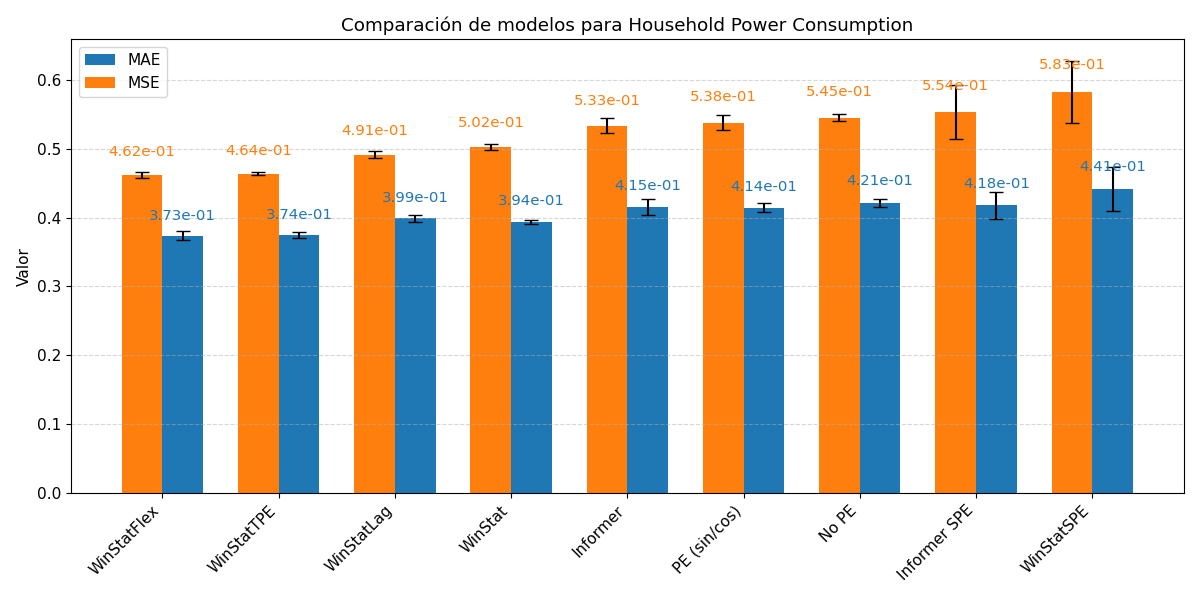
\includegraphics[scale=0.475]{img/hpcgraph}
	\caption{HPC: comparativa gráfica de los positional encodings evaluados}
	\label{hpcgraph}
\end{figure}

En ella, se puede apreciar rápidamente como WinStatFlex y WinStatTPE obtienen el mejor resultado, siendo la variabilidad de T-PE inferior, tal y como indican las barras de error dibujadas.  Informer se sitúa en la parte intermedia de la gráfica, siendo empeorados sus resultados al emplear la codificación fija seno/coseno, no usar codificación, o bien, emplear SPE, el cual ya desestimamos.\\

Si bien todos los modelos propuestos (a excepción de SPE) obtienen mejores resultados frente a Informer, debemos reducir el conjunto de métodos a un número razonable para poder llevar a cabo un experimento similar sobre conjuntos como TINA, de mayor extensión, evitando perder recursos de cómputo en otros PE menos prometedores. Por este motivo, se toma la decisión de continuar únicamente con las alternativas WinStatFlex y WinStatTPE, las cuales han mostrado un buen desempeño en las pruebas realizadas, y ofrecen resultados demasiado cercanos como para discriminar únicamente usando los valores de este conjunto de datos.\\

Y ahora, debemos volver a hacer hincapié sobre el objetivo que estamos persiguiendo: verificar si los nuevos encodings añaden de verdad información semántica. Para ello, realizaremos el experimento anteriormente mencionado del barajado del decoder. Volveremos a ejecutar los dos mejores algoritmos seleccionados e Informer, y ver si realmente se repite la problemática vista en \cite{zeng2022transformerseffectivetimeseries}.\\

En la tabla \ref{hpcresultados_modelos}, podemos encontrar los resultados, del cual podemos extraer varias conclusiones:
\begin{table}[ht]
	\centering
	\begin{tabular}{l|N|N|N|N}
		\toprule
		Modelo & \text{MAE (Media)} & \text{MAE (STD)} & \text{MSE (Media)} & \text{MSE (STD)} \\
		\midrule
		WinStatFlex & 0,373488 & 0,006858 & 0,461892 & 0,004841 \\
		WinStatTPE & 0,374392 & 0,004132 & 0,463651 & 0,001917 \\
		Informer & 0,415272 & 0,012216 & 0,532965 & 0,010976 \\
		No PE & 0,421343 & 0,005856 & 0,544844 & 0,005447 \\
		Informer (Shuffled) & 0,419960 & 0,002769 & 0,548443 & 0,009148 \\
		WinStatFlex (Shuffled) & 0,581124 & 0,021991 & 0,782092 & 0,027368 \\
		WinStatTPE (Shuffled) & 0,581001 & 0,046717 & 0,851115 & 0,024083 \\
		\bottomrule
	\end{tabular}
	\caption{HPC: resultados para experimento de mezcla en encoder}
	\label{hpcresultados_modelos}
\end{table}


\begin{table}[ht]
	\centering
	\begin{tabular}{l|N|N|N|N}
		\toprule
		Modelo & \text{Tº Test(s)} & \text{Tº Test(s)-STD} & \text{Tº Train(s)} & \text{Tº Train(s)-STD} \\
		\midrule
		WinStatFlex & 350,8360 & 5,5675 & 18652,7244 & 128,3429 \\
		WinStatTPE & 296,2529 & 1,9551 & 18913,6335 & 28,7927 \\
		Informer & 91,9412 & 1,2444 & 7817,0202 & 821,2709 \\
		No PE & 125,0538 & 2,8330 & 10382,2665 & 2083,3163 \\
		Informer (Shuffled) & 85,9877 & 0,7681 & 7923,0834 & 1508,2765 \\
		WinStatFlex (Shuffled) & 330,9885 & 6,0409 & 20842,9511 & 1877,7778 \\
		WinStatTPE (Shuffled) & 295,0051 & 1,2049 & 20580,5136 & 2278,5627 \\
		\bottomrule
	\end{tabular}
	\caption{HPC: Tiempos de ejecución para cada modelo tras el mezclado}
	\label{hpc_tiempos_modelos}
\end{table}

\begin{itemize}
	\item En primer lugar, el rendimiento de Informer original y mezclados es muy similar, con una diferencia mínima entre ellos, respaldando así los resultados realizados en el paper original. La versión sin PE se sitúa justo en medio de ambos resultados, haciendo que los 3 modelos ofrezcan de manera general el mismo rendimiento y afianzando la pobre semántica y mantenimiento de orden que aporta la estrategia tradicional.
	\item WinStatFlex sufre de manera marcada el impacto de aplicar el barajado, lo cual son muy buenos resultados. Esto nos indica que la información aportada por este método es capaz de modelar de manera adecuada tanto el contexto como la estructura inherente de la serie, y que cuando se aplica sobre una entrada mezclada, se produce una gran alteración y degradación del rendimiento. Este comportamiento resulta coherente y lógico desde un punto de vista teórico, y sus efectos se aprecian a nivel empírico: el MSE pasa de $0,461892$ a $0,782092$, lo que supone un empeoramiento relativo del 69,3\%.
	\item WinStatTPE muestra un efecto similar; al aplicar el barajado, pasamos de $0,463651$ a $0,851115$, sufriendo incluso un mayor empeoramiento que la variante Flex. En valores relativos, la diferencia es de un 83,5\%, indicando por tanto que la información semántica aportada por T-PE es aún más sensible a barajado que el resto de codificaciones.
\end{itemize}

Estos resultados refuerzan, por tanto, un mejor aprovechamiento del contexto local y semántico de los datos, siendo ahora una parte clave del modelo que se ve tremendamente afectada cuando realizamos alteraciones que manipulen la estructura y rompan el contexto temporal. Gracias a este experimento, hemos podido verificarlo de manera sencilla y poner en valor los resultados obtenidos. Los tiempos de ejecución han crecido, como era de esperar, en los modelos mezclados (representados como variantes \textit{Shuffled} en la tabla \ref{hpc_tiempos_modelos}), pero dicho sobrecoste asociado es asumible dada la utilidad del procedimiento.\\

\begin{figure}[!ht]
	\centering
	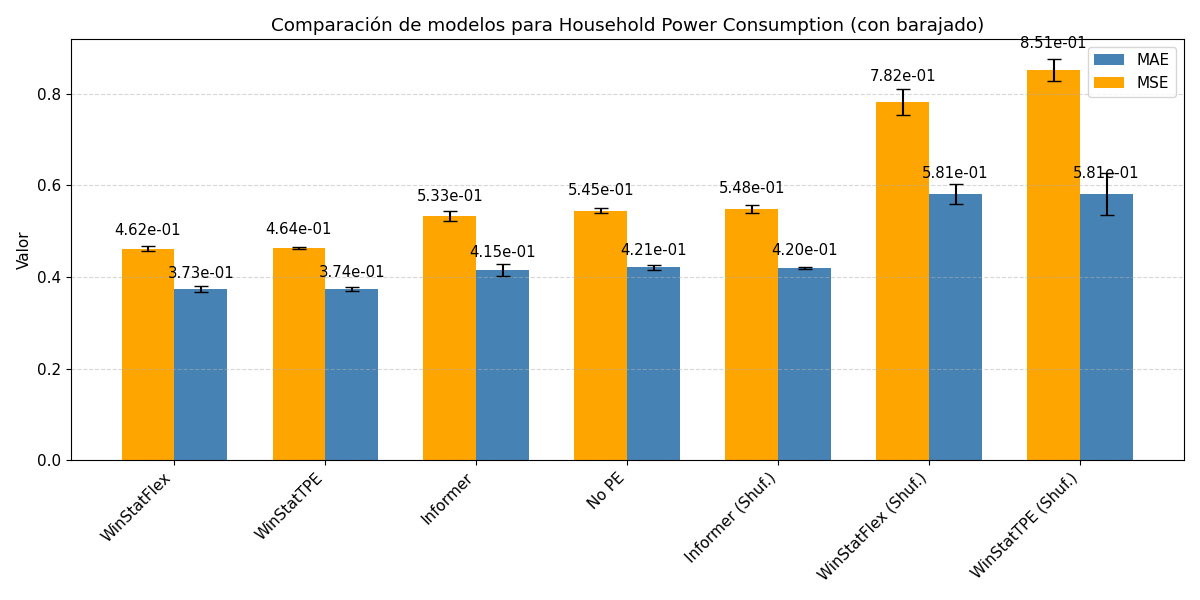
\includegraphics[scale=0.475]{img/hpcgraphshuffled}
	\caption{HPC: comparativa gráfica de los PE, tras aplicar barajado}
	\label{hpcgraphshuffled}
\end{figure}

A modo de resumen final, en la figura \ref{hpcgraphshuffled} se representan los resultados de los modelos comparados con el barajado, para apreciar de manera visual que las diferencias entre pares de modelos ahora son bastante notables en comparación con Informer original.


\subsection{ETT: Evaluación de PE}

ETT será nuestro segundo entorno de pruebas para los encodings. En este caso, escogeremos únicamente las variantes WinStatFlex y WinStatTPE, debido a la decisión tomada en el apartado anterior para filtrar los encodings más diferenciales respecto al modelo de referencia. \\

Este dataset presenta una longitud bastante más reducida que el anterior, especialmente en sus variantes horarias, ya que estas no llegan a las 15.000 mediciones. Sin embargo, resulta interesante realizar las pruebas en esta variante debido a que se trata de uno de los principales conjuntos de referencia en estado del arte, con el objetivo de mostrar la escalabilidad y flexibilidad del modelo al operar tanto en entornos de larga duración como en problemas de extensión más reducida.\\

 Para validar este efecto en diferentes contextos, se realizarán las pruebas sobre los dos transformadores, es decir, sobre los conjuntos de datos \textit{ETTh1} y \textit{ETTh2}, correspondientes a las variantes horarias, con el fin de comprobar si el comportamiento de ambos sistemas, medidos bajo las mismas condiciones, pero con diferentes comportamientos, nos aportan conclusiones similares. Comenzaremos el examen por la variante ETTh1 y posteriormente analizaremos ETTh2 para cada algoritmo.


\subsubsection{Análisis y resultados}

Una vez configurado el entorno de pruebas, podemos pasar a la evaluación del modelo. Al igual que se hizo con HPC, se han fijado todos los parámetros comunes a los algoritmos a los mismos valores con el objetivo de que la configuración de la arquitectura no afecte a los resultados, y sea el propio encoding el que determine la diferencia. La arquitectura y los parámetros asociados se pueden ver en la tabla \ref{ajustesett}. En este caso, el horizonte de predicción y el tamaño de ventana son menores, para así adecuarnos al tamaño de los datos disponibles, y teniendo en cuenta también que la granularidad es horaria.

\begin{table}[!ht]
	\centering
	\begin{tabular}{l|l}
		\toprule
		Parámetro & Valor \\
		\midrule
		{Modelo de atención} & Vanilla \\
		{Tamaño de batch} & 32 \\
		{Dropout} & 0.2 \\
		{Nº de ejecuciones} & 5 \\
		{Tamaño de ventana} & 24 \\
		{Longitud de secuencia} & 96 \\
		{Longitud de etiqueta/contexto} & 48 \\
		{Longitud de predicción} & 24 \\
		\bottomrule
	\end{tabular}
	\caption{ETT: configuración de parámetros comunes empleada para los experimentos}
	\label{ajustesett}
\end{table}

\paragraph{Informer}

Siguiendo el camino establecido, comenzaremos ejecutando Informer, nuestro algoritmo de referencia, incorporando la información de los timestamps mediante timeF. Aunque podríamos tomar los resultados registrados en su publicación original como referencia~\cite{zhou2021informerefficienttransformerlong}, desconocemos los detalles de bajo nivel sobre cómo obtuvieron los resultados finales, por lo que es preferible reejecutar el experimento para realizar una comparativa justa.

\begin{table}[!ht]
	\centering
	\begin{tabular}{l|N|N}
		\toprule
		\text{Métrica} & \text{Media} & \text{STD} \\
		\midrule
		MSE & 0,545807 & 0,020421 \\
		MAE & 0,532375 & 0,017099 \\
		MAPE & 11,799151 & 1,626443 \\
		MSPE & 48779,951562 & 13908,208000 \\
		RMSE & 0,738659 & 0,013775 \\
		TrainTime(s) & 16,819558 & 1,748976 \\
		TestTime(s) & 0,383596 & 0,002506 \\
		\bottomrule
	\end{tabular}
	\caption{ETTh1: métricas de rendimiento para Informer}
	\label{etth1informer}
\end{table}


\begin{table}[!ht]
	\centering
	\begin{tabular}{l|N|N}
		\toprule
		\text{Métrica} & \text{Media} & \text{STD} \\
		\midrule
		MSE & 0,886627 & 0,100092 \\
		MAE & 0,754907 & 0,053964 \\
		MAPE & 5,925552 & 0,645586 \\
		MSPE & 2924,225586 & 475,51672 \\
		RMSE & 0,940080
		 & 0,053635 \\
		TrainTime(s) & 18,676547 & 1,945601 \\
		TestTime(s) & 0,449962 & 0,024086 \\
		\bottomrule
	\end{tabular}
	\caption{ETTh2: métricas de rendimiento para Informer}
	\label{etth2informer}
\end{table}




En la tabla \ref{etth1informer}, se recogen los resultados de las métricas para ETTh1. Podemos observar que, al igual que en HPC, las métricas distintas a MSE y MAE ofrecen un comportamiento bastate extremo, con tasas de error muy elevadas, potenciadas de nuevo por la cercanía a cero de buena parte de los valores, al estar estos normalizados y tener la serie extremos máximos bastante elevados. Si tomamos como referencia el MSE, obtenemos un valor bastante estable en cuanto a variabilidad del resultado, y con valor próximo al MAE.\\

En el caso de ETTh2 (tabla \ref{etth2informer}), los resultados son bastante diferentes, siendo las métricas de error superiores en valor. Por ejemplo, el MSE es de $0,886$, mientras que el MAE es de $0,7549$. Pero, aunque las variables de ambos fenómenos sean las mismas y compartan unidades de medición, sus comportamientos difieren notablemente, como se evidenció en el análisis realizado en capítulos anteriores. Por ello, realizar una comparación directa de los valores numéricos podría inducir a conclusiones erróneas. Estudiaremos si ambos mejoran o empeoran cuando se usa otra codificación, pero con respecto a sí mismos y no entre ellos.\\

Obtenida ya la primera referencia, procederemos a revisar el resto de encodings para determinar empíricamente si este resultado es bueno o puede ser mejorable.
 
 
\paragraph{PE sinusoidal}
 
 Para volver a comprobar si la pequeña información de contexto proporcionada por timeF es relevante, reejecutaremos la implementación de informer eliminando dicha componente y ejecutando únicamente con la parte geométrica del encoding.\\
  
 \begin{table}[!ht]
 	\centering
 	\begin{tabular}{l|N|N}
 		\toprule
 		\text{Métrica} & \text{Media} & \text{STD} \\
 		\midrule
	 	MSE & 0,577572 & 0,075510 \\
		MAE & 0,555214 & 0,053092 \\
		MAPE & 11,869595 & 1,172958 \\
		MSPE & 47931,058203 & 10247,69 \\
		RMSE & 0,758369 & 0,049472 \\
		TrainTime(s) & 25,520506 & 0,385055 \\
		TestTime(s) & 0,607528 & 0,003783 \\
 		\bottomrule
 	\end{tabular}
 	\caption{ETTh1: resultados para encoding seno-coseno}
 	\label{etth1fixed}
 \end{table}
 
 
  
 \begin{table}[!ht]
 	\centering
 	\begin{tabular}{l|N|N}
 		\toprule
 		\text{Métrica} & \text{Media} & \text{STD} \\
 		\midrule
 		MSE & 1,388127 & 0,158151 \\
		MAE & 0,935477 & 0,051373 \\
		MAPE & 3,730952 & 0,198797 \\
		MSPE & 1794,159741 & 267,398770 \\
		RMSE & 1,176358 & 0,065637 \\
		TrainTime(s) & 18,290615 & 0,414452 \\
		TestTime(s) & 0,465952 & 0,039954 \\
 		\bottomrule
 	\end{tabular}
 	\caption{ETTh2: resultados para encoding seno-coseno}
 	\label{etth2fixed}
 \end{table}
 
  Atendiendo a los valores dados por la tabla \ref{etth1fixed} para ETTh1, esta vez sí que encontramos una diferencia notable entre el modelo original y este; en el MSE encontramos una diferencia de 0,032 (0,545807 vs 0,577572), mientras que en MAE ronda una diferencia de 0,02 (valor de 0,532375 vs 0,555214). Por lo tanto, parece que la información aportada por dicha componente de Informer parece aportar información relevante.\\
  
  Por otro lado, en el caso del segundo dataset, estamos ante un caso bastante curioso, ya que se ha producido un aumento bastante considerable en los valores de toda las métricas; en el caso de MSE, la diferencia es de 0,5, bastante alta, mientras que en MAE es de 0,38. Esto nos está indicando que el segundo dataset sea posiblemente más complejo de modelar, y se requiera un mayor contexto para modelar adecuadamente el comportamiento. De esta forma, sería razonable pensar que cuando apliquemos las propuestas Flex y TPE, el salto de rendimiento sea considerable.\\
  
  En definitiva, este modelo difiere en comportamiento considerablemente entre los dos conjuntos de datos. En el caso de ETTh1, se obtiene una mejora del 5,8\%, mientras que en el caso de ETTh2, se obtiene un empeoramiento relativo del 56,5\%, siendo una degradación considerable.
 
 \paragraph{WinStatFlex}
 
Ahora procedemos a evaluar WinStatFlex, para ver si conseguimos mejorar los resultados, de referencia gracias al enfoque flexible de la ponderación, en ambos datasets.
\begin{table}[!ht]
	\centering
	\begin{minipage}{0.5\textwidth}
		\centering
		\begin{tabular}{l|N|N}
			\toprule
			\text{Métrica} & \text{Media} & \text{STD} \\
			\midrule
			MSE & 0,467676 & 0,101775 \\
			MAE & 0,512808 & 0,065133 \\
			MAPE & 3,343877 & 0,767829 \\
			MSPE & 1530,202856 & 410,789550 \\
			RMSE & 0,679749 & 0,074946 \\
			TrainTime(s) & 32,989481 & 3,775380 \\
			TestTime(s) & 0,834729 & 0,024313 \\
			\bottomrule
		\end{tabular}
	\end{minipage}%
	\hfill
	\begin{minipage}{0.4\textwidth}
		\centering
			\begin{tabular}{l|N}
			\toprule
			Componente & \text{Peso aprendido} \\
			\midrule
			Stats & 0,2704 \\
			PE & 0,2506 \\
			LPE & 0,242 \\
			tAPE & 0,2371 \\
			\bottomrule
		\end{tabular}
	\end{minipage}
	
	\caption{ETTh1: resultados para encoding WinStatFlex}
	\label{etth1flex}
\end{table}


Comenzando por los resultados de ETTh1, podemos destacar los siguientes aspectos:

\begin{itemize}
	\item El rendimiento obtenido, tomando como referencia la métrica MSE, da salto considerable hacia delante. En comparación con el modelo Informer original, se ha logrado una mejora absoluta de casi $0,08$, equivalente a un 17,1\% de mejora. Este incremento es bastante alto, considerando el rango de valores en el que nos situamos. Estos resultados reafirman la potencia de la combinación mediante pesos entrenables más allá del dataset visto anteriormente.
	\item El tiempo de ejecución no se ha visto especialmente afectado en aspectos absolutos, ya que el incremento en tiempo es de apenas 16 segundos. Sin embargo a nivel relativo es considerable, ya que estamos hablando de que es doble del tiempo Informer.
	\item Los valores de los pesos son bastante equilibrados en esta ocasión, aunque se muestra un mayor inclinación por la información apropiada por la ventana de estadísticos y las diferencias de lags, la cual es un 27,04\% de la suma final. tAPE es el método absoluto de codificación menos valorados, aunque con escasa diferencia de su valor inicial de 0,25.
\end{itemize}


Por otro lado, tenemos el comprotamiento de ETTh2, el cual también muestra mejoras notables, incluso de mayor relevancia:


\begin{table}[!ht]
	\centering
	\begin{minipage}{0.5\textwidth}
		\centering
			\begin{tabular}{l|N|N}
				\toprule
				\text{Métrica} & \text{Media} & \text{STD} \\
				\midrule
			MSE & 0,465990 & 0,027734 \\
			MAE & 0,494661 & 0,019507 \\
			MAPE & 10,515547 & 0,347335 \\
			MSPE & 40193,949219 & 2941,565400 \\
			RMSE & 0,682334 & 0,020266 \\
			TrainTime(s) & 27,822449 & 2,565389 \\
			TestTime(s) & 0,779390 & 0,008920 \\
			\bottomrule
		\end{tabular}
	\end{minipage}%
	\hfill
	\begin{minipage}{0.4\textwidth}
		\centering
			\begin{tabular}{l|N}
			\toprule
			Componente & \text{Peso aprendido} \\
			\midrule
			Stats & 0,2569 \\
			PE & 0,2504 \\
			LPE & 0,2513 \\
			tAPE & 0,2413 \\
			\bottomrule
		\end{tabular}
	\end{minipage}
	
	\caption{ETTh2: resultados para encoding WinStatFlex}
	\label{etth2flex}
\end{table}
 
 
 \begin{itemize}
 	\item El incremento en rendimiento es muy marcado: hemos pasado del bajo rendimiento del enfoque seno-coseno, a obtener una mejora de aproximadamente 0,42 de MSE con respecto a Informer. En términos relativos, es una mejora del resultado del 90,3\%, indicando que hemos reducido casi a la mitad el error medio. El bajo valor de la desviación además refuerza que este resultado es fácilmente reproducible.
 	
 	\item Aunque el tiempo de ejecución ha aumentado, podemos considerarlo un sobrecoste razonable, dado que hemos logrado casi duplicar el rendimiento sin duplicar el tiempo de entrenamiento. Por tanto, este incremento resulta asumible y no representa un inconveniente significativo.
 	
 	\item El valor final de los pesos (tabla derecha de \ref{etth1flex}) es bastante equilibrado. Prácticamente, los valores han permanecido iguales al valor de partida, que recordemos que era 0,25 para cada uno de ellos. Por lo tanto, parece que las 4 componentes aportan información útil de manera equilibrada. Incluso TAPE, anteriormente en HPC la minoritaria, parece aportar información vinculante.
 \end{itemize}
 
 En definitiva, el uso de WinStatFlex ha resultado muy positivo en este conjunto de datos, proporcionando un notable aumento de rendimiento en ambos conjuntos, y especialmente en ETTh2, que parece reflejar una mayor complejidad en su modelado en comparación con ETTh1. En ambos casos, es llamativo el escaso ajuste de los pesos de ponderación respecto a los valores iniciales, lo cual podría deberse a que la cantidad de datos disponible es relativamente limitada y el entrenamiento se interrumpe pronto debido al early stopping. No obstante, esto no indica que este método de codificación sea inadecuado; por el contrario, demuestra que WinStatFlex también se adapta a conjuntos de datos cortos.
 
 \paragraph{WinStatTPE}
 
 La variante de WinStat con T-PE ha sido el siguiente encoding probado empíricamente. 
 \begin{table}[!ht]
 	\centering
 	\begin{minipage}{0.5\textwidth}
 		\centering
 		\begin{tabular}{l|N|N}
 			\toprule
 			\text{Métrica} & \text{Media} & \text{STD} \\
 			\midrule
 			MSE & 0,489647 & 0,048151 \\
	 		MAE & 0,507179 & 0,031240 \\
	 		MAPE & 11,085088 & 0,730064 \\
	 		MSPE & 45770,907813 & 7129,339000 \\
	 		RMSE & 0,698881 & 0,034805 \\
	 		TrainTime(s) & 52,732013 & 0,954233 \\
	 	 	TestTime(s) & 1,339969 & 0,043272 \\
 			\bottomrule
 		\end{tabular}
 	\end{minipage}%
 	\hfill
 	\begin{minipage}{0.4\textwidth}
 		\centering
 			\begin{tabular}{l|N}
 			\toprule
 			Componente & \text{Peso aprendido} \\
 			\midrule
 			Stats & 0,258 \\
 			PE & 0,247 \\
 			LPE & 0,232 \\
 			TPE & 0,263 \\
 			\bottomrule
 		\end{tabular}
 	\end{minipage}
 	
 	\caption{ETTh1: resultados para encoding WinStatTPE}
 	\label{etth1tpe}
 \end{table}
 
 Procediendo de la manera habitual, comenzaremos analizando primero ETTh1 (tabla \ref{etth1tpe}):
 
 \begin{itemize}
 	\item Nuestra métrica de referencia, MSE, muestra un rendimiento bastante cercano a la variante Flex, aunque ligeramente inferior. Si bien la diferencia con respecto a Informer sigue siendo notable, de $0,1146$, el desempeño frente a WinStatFlex resulta inferior en todas las demás métricas. Sin embargo, la varianza, uno de los puntos fuertes de T-PE, se mantiene especialmente en el cálculo del MSE, lo que sugiere que sigue siendo un elemento clave de esta variante.
 	
 	\item El tiempo de ejecución ha crecido hasta valores demasiado elevados, muy cercanos al minuto de duración. Si bien en conjuntos como este sigue siendo un tiempo bajo, estamos ante un algoritmo que ofrece un menor rendimiento que WinStatFlex, pero un tiempo 20 segundos superior, por lo que su utilización no se motivada en cuanto al equilibrio métricas-rendimiento.
 	\item Los valores de los pesos vuelven a ser prácticamente equilibrados, siguiendo las tendencias vistas hasta ahora.
 \end{itemize}
 
 Para ETTh2, la tónica es bastante similar (ver tabla \ref{etth2tpe}); las métricas reflejan un empeoramiento de los resultados en todas las medidas, destacando el 0,5963 de MSE, y el tiempo de ejecución es de 54 segundos de media, aumentando así considerablemente el coste de entrenar este modelo. Por lo tanto, el modelado del segundo transformador tiene un comportamiento similar a ETTh1, y WinStatTPE parece no adaptarse del todo a sus condiciones.
 
  \begin{table}[!ht]
 	\centering
 	\begin{minipage}{0.5\textwidth}
 		\centering
 		\begin{tabular}{l|N|N}
 			\toprule
 			\text{Métrica} & \text{Media} & \text{STD} \\
 			\midrule
 			MSE & 0,596380 & 0,076012 \\
 			MAE & 0,588919 & 0,049605 \\
 			MAPE & 4,052313 & 0,355036 \\
 			MSPE & 1707,383569 & 527,479550 \\
 			RMSE & 0,770738 & 0,048395 \\
  			TrainTime(s) & 54,832880 & 4,593619 \\
 			TestTime(s) & 1,327944 & 0,068589 \\
 			\bottomrule
 		\end{tabular}
 	\end{minipage}%
 	\hfill
 	\begin{minipage}{0.4\textwidth}
 		\centering
 			\begin{tabular}{l|N}
 			\toprule
 			Componente & \text{Peso aprendido} \\
 			\midrule
 			Stats & 0,251 \\
 			PE & 0,249 \\
 			LPE & 0,249 \\
 			TPE & 0,251 \\
 			\bottomrule
 		\end{tabular}
 	\end{minipage}
 	
 	\caption{ETTh2: resultados para encoding WinStatTPE}
 	\label{etth2tpe}
 \end{table}
 
 No obstante, es importante destacar que estos resultados continúan siendo significativamente superiores a los obtenidos con Informer, lo que confirma que hemos alcanzado el objetivo propuesto de mejorar los encodings analizados.
 
 \paragraph{Informer sin PE}
 
 Por último, nos volvemos a plantear de nuevo la siguiente pregunta: ¿marca la diferencia emplear encoding en este conjunto de datos? Aunque ya hemos demostrado teóricamente que siempre será necesario disponer de él, volveremos a comprobar cuál es el impacto de retirar la componente posicional al embedding, tomando como base el modelo Informer.\\
 
  \begin{table}[!ht]
 	\centering
 	\begin{tabular}{l|N|N}
 		\toprule
 		\text{Métrica} & \text{Media} & \text{STD} \\
 		\midrule
 		MSE & 0,923467 & 0,084128 \\
		MAE & 0,741918 & 0,050922 \\
		MAPE & 14,232987 & 4,295049 \\
		MSPE & 76807,512109 & 46287,280000 \\
		RMSE & 0,960007 & 0,043059 \\
		TrainTime(s) & 17,335851 & 3,149851 \\
		TestTime(s) & 0,451098 & 0,043514 \\
 		\bottomrule
 	\end{tabular}
 	\caption{ETTh1: métricas de rendimiento para Informer sin PE}
 	\label{etth1nope}
 \end{table}
 
 
 
   \begin{table}[!ht]
 	\centering
 	\begin{tabular}{l|N|N}
 		\toprule
 		\text{Métrica} & \text{Media} & \text{STD} \\
 		\midrule
 	 	MSE & 1,013217 & 0,241743 \\
 		MAE & 0,777736 & 0,119947 \\
 		MAPE & 6,796825 & 1,558902 \\
 		MSPE & 4086,226156 & 447,778530 \\
 		RMSE & 0,998585 & 0,126672 \\
 		TrainTime(s) & 18,196816 & 2,308764 \\
 	 	MSE & 1,013217 & 0,241743 \\
 		\bottomrule
 	\end{tabular}
 	\caption{ETTh2: métricas de rendimiento para Informer sin PE}
 	\label{etth2nope}
 \end{table}

En ambos casos, el empeoramiento es notable. Para ETTh1, este modelo es el que peores resultados ha obtenido, demostrando así la necesidad indiscutible del encoding, pues ha pasado a aumentar el MSE $0,3776$ (teniendo en cuenta el $0,5458$ de Informer), provocando una caída relativa del rendimiento del 69,2\%.\\

En ETTh2, por su parte, aunque el empeoramiento también es significativo, pasando a obtener $1,013217$ y $0,777736$ de MSE  y MAE, con respecto a los $0,886627$ y $0,754907$ de Informer, respectivamente, resulta curioso ver que aún así, el rendimiento es mejor que empleando únicamente Informer con encoding sinusoidal original sin TimeF. 

\subsubsection{Elección del mejor modelo}

Con todos los algoritmos ejecutados, y sus correspondientes análisis podemos definitivamente escoger el modelo de codificación que mejores resultados ha obtenido. Para contrastarlo también visualmente, se han creado los gráficos \ref{etth1fin} y \ref{etth2fin} (así como las tablas \ref{etth1fintab} y \ref{etth2fintab}), los cuales recogen los resultados de los subconjuntos ETTh1 y ETTh2, respectivamente, ordenados de mejor a peor resultado. En ambos, se muestran también los resultados de barajar la entrada del decoder tanto para WinStatFlex como para WinStatTPE.\\


\begin{figure}[!ht]
	\centering
	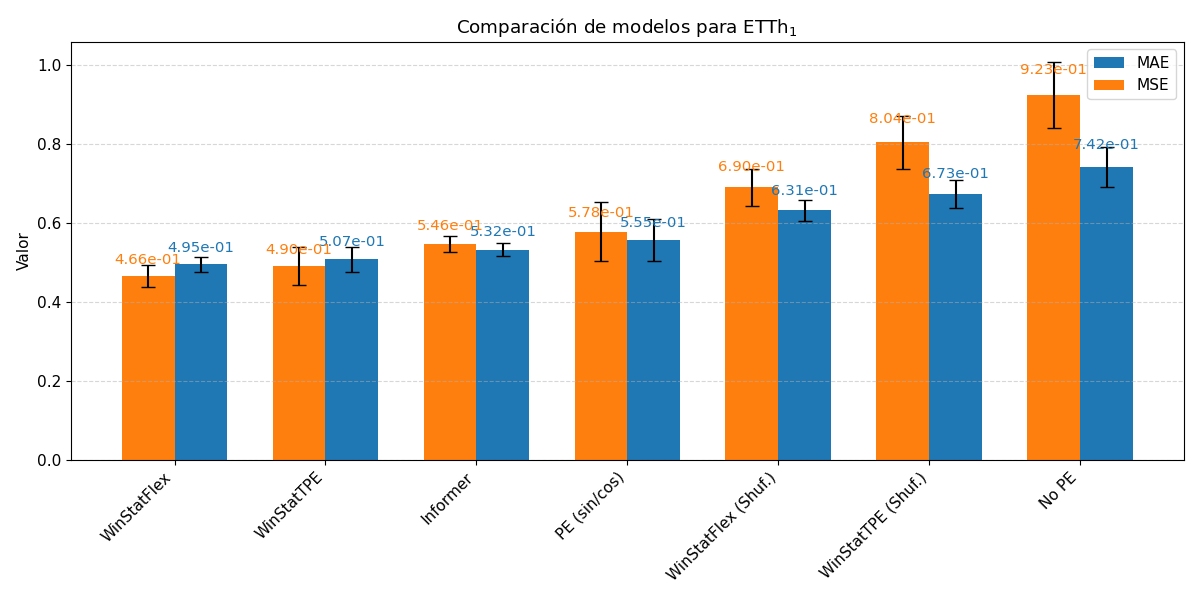
\includegraphics[scale=0.475]{img/etth1fin}
	\caption{ETTh1: comparativa gráfica de los positional encodings evaluados}
	\label{etth1fin}
\end{figure}

\begin{table}[ht]
	\centering
	\begin{tabular}{l|N|N|N|N}
		\toprule
		Modelo & \text{MAE (Media)} & \text{MAE (STD)} & \text{MSE (Media)} & \text{MSE (STD)} \\
		\midrule
		WinStatFlex            & 0.4947 & 0.0195 & 0.4660 & 0.0277 \\
		WinStatTPE             & 0.5072 & 0.0312 & 0.4896 & 0.0482 \\
		Informer               & 0.5324 & 0.0171 & 0.5458 & 0.0204 \\
		PE (sin/cos)           & 0.5552 & 0.0531 & 0.5776 & 0.0755 \\
		WinStatFlex (Shuf.)    & 0.6313 & 0.0276 & 0.6897 & 0.0461 \\
		WinStatTPE (Shuf.)     & 0.6728 & 0.0358 & 0.8036 & 0.0667 \\
		No PE                  & 0.7419 & 0.0509 & 0.9235 & 0.0841 \\
		\bottomrule
	\end{tabular}
	\caption{ETTh1: resultados ordenados, incluyendo modelos barajados}
	\label{etth1fintab}
\end{table}

\begin{figure}[!ht]
	\centering
	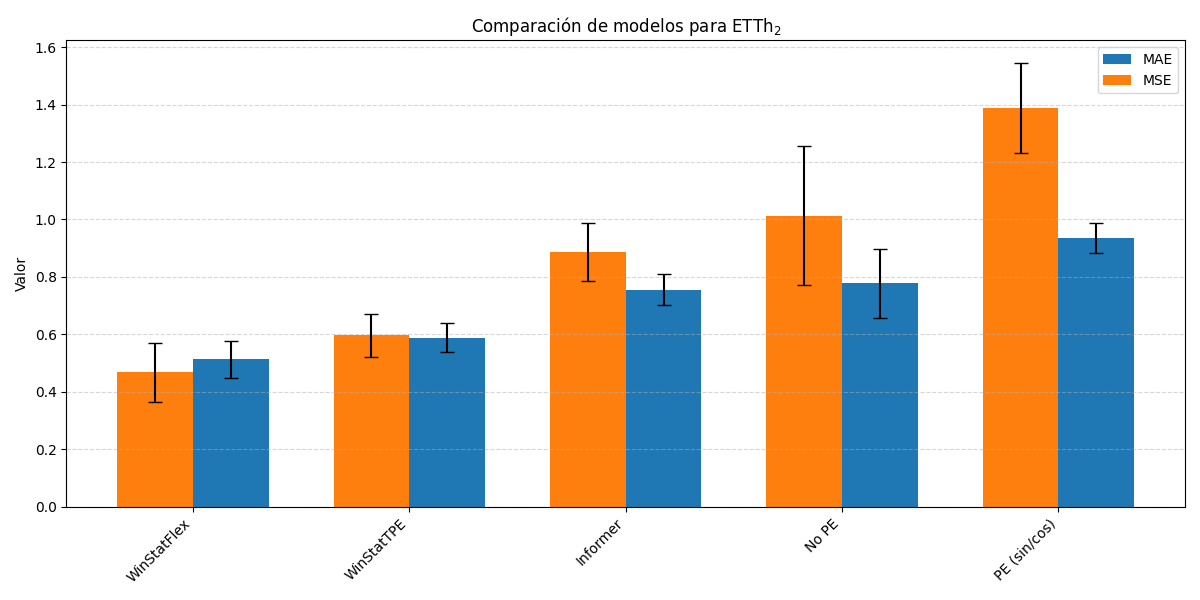
\includegraphics[scale=0.475]{img/etth2fin}
	\caption{ETTh2: comparativa gráfica de los positional encodings evaluados}
	\label{etth2fin}
\end{figure}




\begin{table}[ht]
	\centering
	\begin{tabular}{l|N|N|N|N}
		\toprule
		Modelo & \text{MAE (Media)} & \text{MAE (STD)} & \text{MSE (Media)} & \text{MSE (STD)} \\
		\midrule
		WinStatFlex            & 0.5128 & 0.0651 & 0.4677 & 0.1018 \\
		WinStatTPE             & 0.5889 & 0.0496 & 0.5964 & 0.0760 \\
		WinStatTPE (Shuf.)     & 0.6892 & 0.0714 & 0.8294 & 0.1418 \\
		WinStatFlex (Shuf.)    & 0.6929 & 0.0671 & 0.8608 & 0.1625 \\
		Informer               & 0.7549 & 0.0540 & 0.8866 & 0.1001 \\
		No PE                  & 0.7777 & 0.1199 & 1.0132 & 0.2417 \\
		PE (sin/cos)           & 0.9355 & 0.0514 & 1.3881 & 0.1582 \\
		\bottomrule
	\end{tabular}
	\caption{ETTh2: resultados ordenados, incluyendo modelos barajados}
	\label{etth2fintab}
\end{table}




Se puede observar claramente que WinStatFlex y WinStatTPE alcanzan los mejores resultados, destacando especialmente el primero. Informer, en cambio, ofrece un desempeño intermedio, que se ve reducido cuando se emplea la codificación fija de senos/cosenos, pero es mejor a la hora de prescindir de cualquier encoding. La magnitud de estas diferencias se vuelve aún más evidente en el segundo conjunto de datos, tal y como se mostró numéricamente en el subpunto anterior.\\

En el subconjunto ETTh1, podemos ver que el barajado de las dos propuestas analizadas, a pesar de empeorar gravemente los resultados tanto para MAE como para MSE (aumentándolos en $0,2$ en ambos métricas para Flex; 0,31 y 0,169 para MSE y MAE de la variante T-PE, respectivamente) sigue ofreciendo mejores resultados que no utilizar ningún tipo de codificación. Este comportamiento resulta interesante, ya que normalmente podríamos esperar que desordenar la información semántica dificultara aún más el aprendizaje que no disponer de ella.\\

En el caso de ETTh2 resalta especialmente el pésimo rendimiento de la codificación sinusoidal, siendo esta peor incluso que los modelos con codificación y semántica barajadas. Es posible que, en ese conjunto de datos concreto, la inclusión de senos y cosenos pueda introducir información posicional que no se alinea perfectamente con las relaciones temporales reales de la serie, y afecte negativamente la capacidad del modelo para capturar patrones relevantes cuando no se complementa adecuadamente con otros mecanismos. Al omitir cualquier PE, el modelo parece aprender directamente de la estructura pura de los datos, y se ve menos afectado por este problema.\\

En conclusión, estos resultados ponen en valor y refuerzan la necesidad de un encoding flexible y con gran capacidad semántica y local, que permita al modelo adaptarse correctamente a su estructura, incluso en conjuntos menos extensos como este. WinStatFlex consigue el mejor resultado como prueba de ello.

\subsection{Yellow Trip Data: Evaluación de PE}

Yellow Trip será el tercer conjunto de datos empleado para evaluar el rendimiento de las propuestas de encoding. A diferencia de los dos datasets anteriores, este presenta un cambio significativo en el contexto semántico, pues se abandona el entorno de los sistemas eléctricos para centrarse en los taxis de Nueva York. Además de su distinta naturaleza, marcada por una estacionalidad más pronunciada, resulta relevante la característica previamente señalada: los datos fueron ampliados de manera artificial. \\

Aunque esta expansión podría parecer beneficiosa desde el punto de vista del entrenamiento, pues disponemos de un conjunto más extenso, también podría generar sesgos. Esto se debe a que la serie probablemente fue aumentada mediante modelos predictivos, que, como hemos estudiado a lo largo de este trabajo, tienden a simplificar excesivamente los patrones originales. Por tanto, es posible que los resultados obtenidos con este dataset sean especialmente optimistas, ya que Informer, será capaz de modelarlo de manera fiel, arrojando tasas de error muy bajas.\\

En los siguientes apartados, analizaremos los resultados, teniendo especial cuidado con la escala del MSE y contrastando con el error absoluto con los resultados sean confusos.

\subsubsection{Análisis y resultados}

Una vez presentados los aspectos relevantes, podemos pasar a realizar las ejecuciones. Ante de comenzar, fijaremos todos los parámetros de la arquitectura, tal y como venimos haciendo hasta el momento. En la tabla \ref{ajustestaxi}, se muestra la configuración, la cual es bastante similar a la vista en HPC, pues a nivel estructural, ambos conjuntos muestran una dimensionalidad similar, aunque con la diferencia de que en este caso los datos son de intervalo horario y no minuto a minuto. Recuperamos, por tanto, una mayor longitud de secuencia (180), y un mayor tamaño de ventana (60), de forma que podamos captar la localidad de los datos correctamente.

\begin{table}[!ht]
	\centering
	\begin{tabular}{l|l}
		\toprule
		Parámetro & Valor \\
		\midrule
		{Modelo de atención} & Vanilla \\
		{Tamaño de batch} & 32 \\
		{Dropout} & 0.2 \\
		{Nº de ejecuciones} & 3 \\
		{Tamaño de ventana} & 60 \\
		{Longitud de secuencia} & 180 \\
		{Longitud de etiqueta/contexto} & 60 \\
		{Longitud de predicción} & 60 \\
		\bottomrule
	\end{tabular}
	\caption{Yellow Trip data: configuración de parámetros comunes empleada para los experimentos}
	\label{ajustestaxi}
\end{table}

Los modelos evaluados serán los habituales: Informer, Informer sin PE, Informer con codificación seno-coseno, WinStatFlex, WinStatTPE, y las variantes barajadas de estos dos últimos con vistas al análisis final.

\paragraph{Informer}

Comenzaremos con la ejecución del modelo de partida, Informer. Al igual que en los casos anteriores, la ejecución se realiza empleando la configuración de entrada dada por timeF, y sus correspondientes 3 ejecuciones para obtener el promedio. En la tabla \ref{taxiinformer}, se muestran los resultados obtenidos para esta configuración. 

Como ya se adelantaba en la introducción de este experimento, las métricas están en una escala muy baja, del orden de $10^{-5}$ para el MSE y $10^{-3}$ para MAE. El resto de métricas también se han visto afectadas por este escalado, aunque muestran sorprendentemente valores razonables; por ejemplo, RMSE muestra valores muy cercanos a MAE. No podemos decir lo mismo del tiempo, que en este caso es bastante alto, con un promedio de $13989$ segundos (aproximadamente 3,9 horas).

\begin{table}[!ht]
	\centering
	\begin{tabular}{l|c|c}
		\toprule
		Métrica & Media & STD \\
		\midrule
		MSE & $1,9 \times 10^{-5}$ & $7,0 \times 10^{-6}$ \\
		MAE & $3,987 \times 10^{-3}$ & $7,95 \times 10^{-4}$ \\
		MAPE & $3,902 \times 10^{-2}$ & $9,835 \times 10^{-3}$ \\
		MSPE & $1,833 \times 10^{-3}$ & $1,036 \times 10^{-3}$ \\
		RMSE & $4,259 \times 10^{-3}$ & $8,18 \times 10^{-4}$ \\
		TrainTime(s) & $1,399 \times 10^{4}$ & $5,935 \times 10^{3}$ \\
		TestTime(s) & $8,254 \times 10^{1}$ & $5,489 \times 10^{0}$ \\
		\bottomrule
	\end{tabular}
	\caption{Yellow Trip data: métricas de rendimiento para Informer}
	\label{taxiinformer}
\end{table}

\paragraph{PE sinusoidal}

Para evaluar el rendimiento de un modelo de Transformer casi puramente vanilla, procedemos a realizar el mismo experimento, pero empleando codificación tradicional de tipo seno-coseno. El resultado, como era razonable, se ve afectado negativamente por este cambio (tabla \ref{taxipe}), ya que hemos eliminado prácticamente toda la información relativa a la componente temporal, más allá de la información de posición absoluta aportada por la geometría.\\

A pesar de que la escala se encuentra en valores pequeños, la diferencia de error no es especialmente exagerada, pues empeoramos un 26\% el error en MSE. Si nos fijamos en MAE, algo más estable ante escalas tan pequeñas, podemos ver que también muestra un peor valor, confirmando la tendencia. Sin embargo, sí que es importante destacar que la desviación de los resultados si es considerablemente más alta, indicando que los resultados no son igual de estables numéricamente que en la proposición original de Informer, y se obtiene una peor convergencia.\\

\begin{table}[!ht]
	\centering
	\begin{tabular}{l|c|c}
		\toprule
		Métrica & Media & STD \\
		\midrule
		MSE & $2,4 \times 10^{-5}$ & $1,0 \times 10^{-5}$ \\
		MAE & $4,307 \times 10^{-3}$ & $1,044 \times 10^{-3}$ \\
		MAPE & $3,929 \times 10^{-2}$ & $5,720 \times 10^{-3}$ \\
		MSPE & $1,740 \times 10^{-3}$ & $3,010 \times 10^{-4}$ \\
		RMSE & $4,718 \times 10^{-3}$ & $1,149 \times 10^{-3}$ \\
		TrainTime(s) & $1,594 \times 10^{4}$ & $4,134 \times 10^{3}$ \\
		TestTime(s) & $1,330 \times 10^{2}$ & $1,084 \times 10^{1}$ \\
		\bottomrule
	\end{tabular}
	\caption{Yellow Trip data: métricas de rendimiento para codificación sen/cos}
	\label{taxipe}
\end{table}

\paragraph{WinStatFlex}

Tras el análisis de los modelos ya conocidos en el estado del arte, volvemos a evaluar los modelos propuestos en el trabajo. En este caso, veremos WinStatFlex, el cual obtiene los resultados de la tabla \ref{taxiflex}.\\

Podemos apreciar que los valores obtenidos para todas las métricas resultan un mejora considerable sobre el encoding por defecto de Informer, y reduciendo el error en 0,02. Sin embargo, esta diferencia no es tan marcada como en los conjuntos de datos anteriores. En el MAE si que es mucho más apreciable, ya que se mejora de manera relativa un casi 13\% ($0,458 \times 10^{-3}$ menos). Los pesos dan una mayor importancia a tAPE~\ref{taxiflexpesos} (27,98\%) y reducen ligeramente la relevancia de LPE (24,09\%).\\ 



\begin{table}[!ht]
	\centering
	\begin{tabular}{l|c|c}
		\toprule
		Métrica & Media & STD \\
		\midrule
		MSE & $1,7 \times 10^{-5}$ & $8,0 \times 10^{-6}$ \\
		MAE & $3,529 \times 10^{-3}$ & $1,027 \times 10^{-3}$ \\
		MAPE & $3,885 \times 10^{-2}$ & $1,358 \times 10^{-2}$ \\
		MSPE & $2,482 \times 10^{-3}$ & $1,715 \times 10^{-3}$ \\
		RMSE & $3,964 \times 10^{-3}$ & $9,70 \times 10^{-4}$ \\
		TrainTime(s) & $1,379 \times 10^{4}$ & $3,978 \times 10^{3}$ \\
		TestTime(s) & $1,269 \times 10^{2}$ & $2,414 \times 10^{-1}$ \\
		\bottomrule
	\end{tabular}
	\caption{Yellow Trip data: métricas de rendimiento para codificación WinStatFlex}
	\label{taxiflex}
\end{table}

En cuanto al tiempo de entrenamiento, resulta interesante observar que, a pesar de que este modelo debe computar toda la información contextual para el embedding y podría considerarse más costoso que Informer, el tiempo registrado es menor. Dado que todos los experimentos se ejecutaron en el mismo equipo, esta diferencia podría explicarse por una mejor inicialización de los valores, o bien, por una mayor capacidad de convergencia del modelo, que compensa el sobrecoste inicial derivado de la creación del embedding. Para comprobarlo, simplemente basta con examinar el número de épocas antes de detenerse de cada uno de ellos, donde podemos ver que Informer ha requerido una media de 9 épocas y WinStatFlex, 7, indicando que parte de esta diferencia puede provenir la velocidad de convergencia. 

\begin{table}[!ht]
	\centering
	\begin{tabular}{l|N}
	\toprule
	Componente & \text{Peso aprendido} \\
	\midrule
	Stats & 0,2657 \\
	PE & 0,2137 \\
	LPE & 0,2409 \\
	tAPE & 0,2798 \\
	\bottomrule
\end{tabular}
	\caption{Yellow Trip data: valores aprendidos en los pesos del encoding WinStatFlex}
\label{taxiflexpesos}
\end{table}

\paragraph{WinStatTPE}

Nuestra siguiente prueba emplea el encoding ponderado de TPE, WinStatTPE. La tabla \ref{taxitpe} recoge todos los resultados, mostrando un rendimiento superior a todos los modelos anteriormente evaluados en todas las métricas, y sobre todo en MAE y MSE, que son un 90\% y un 56,5\% mejores que Informer, respectivamente. La reducida varianza de T-PE, ya visualizada en los tres conjuntos anteriores, vuelve a manifestarse constituyendo la principal causa del buen resultado del modelo. El promedio de las ejecuciones presenta una desviación muy pequeña, fruto de la consistencia observada en cada una de las tres iteraciones, y proporciona un rendimiento altamente estable para este conjunto de dato de baja magnitud numérica.\\

\begin{table}[!ht]
	\centering
	\begin{tabular}{l|c|c}
		\toprule
		Métrica & Media & STD \\
		\midrule
		MSE & $1,0 \times 10^{-5}$ & $5,0 \times 10^{-6}$ \\
		MAE & $2,547 \times 10^{-3}$ & $9,37 \times 10^{-4}$ \\
		MAPE & $4,867 \times 10^{-2}$ & $3,270 \times 10^{-2}$ \\
		MSPE & $1,290 \times 10^{-2}$ & $1,578 \times 10^{-2}$ \\
		RMSE & $3,009 \times 10^{-3}$ & $9,54 \times 10^{-4}$ \\
		TrainTime(s) & $5,893 \times 10^{4}$ & $2,992 \times 10^{4}$ \\
		TestTime(s) & $4,151 \times 10^{2}$ & $2,353 \times 10^{0}$ \\
		\bottomrule
	\end{tabular}
	\caption{Yellow Trip data: métricas de rendimiento para codificación WinStatTPE}
	\label{taxitpe}
\end{table}


\begin{table}[!ht]
	\centering
		\begin{tabular}{l|N}
		\toprule
		Componente & \text{Peso aprendido} \\
		\midrule
		Stats & 0,278 \\
		PE & 0,238 \\
		LPE & 0,202 \\
		TPE & 0,282 \\
		\bottomrule
	\end{tabular}
	\caption{Yellow Trip data: valores aprendidos en los pesos del encoding WinStatTPE}
	\label{taxitpepesos}
\end{table}

La proporción de pesos escogida parece ser considerablemente diferente a la variante que usa tAPE, ya que en este caso, una de las componentes más afectadas en el PE aprendible, que desciende su relevancia en la suma final hasta el $20,2\%$, y T-PE adquiere el papel protagonista, siendo la componente de mayor valor (28,2\%) en términos relativos.\\

Por último, el tiempo de ejecución puede indicar un posible punto débil del modelo, ya que es 4,5 veces mayor al empleado por Informer y algo más que eso en el caso de WinStatFlex. Ante dicho aumento de coste, la viabilidad de este algoritmo podría no estar justificada si el tiempo de entrenamiento y ajuste fuera crítico. Pero, en este caso, se busca modelar comportamientos altamente estacionales y no se requiere una ejecución a tiempo real, por lo que esta limitación realmente no es tan decisivo, motivando, a pesar del sobrecoste, su utilización.

\paragraph{Informer sin PE}

Para cerrar la fase de evaluación, probaremos con el modelo sin codificación temporal, a modo de algoritmo base que, teóricamente, debe ofrecer el peor rendimiento.

\begin{table}[!ht]
	\centering
	\begin{tabular}{l|c|c}
		\toprule
		Métrica & Media & STD \\
		\midrule
		MSE & $4,6 \times 10^{-5}$ & $6,0 \times 10^{-5}$ \\
		MAE & $4,626 \times 10^{-3}$ & $3,954 \times 10^{-3}$ \\
		MAPE & $4,494 \times 10^{-2}$ & $3,426 \times 10^{-2}$ \\
		MSPE & $3,702 \times 10^{-3}$ & $3,965 \times 10^{-3}$ \\
		RMSE & $5,113 \times 10^{-3}$ & $4,488 \times 10^{-3}$ \\
		TrainTime(s) & $2,288 \times 10^{4}$ & $8,549 \times 10^{3}$ \\
		TestTime(s) & $1,063 \times 10^{2}$ & $9,637 \times 10^{-1}$ \\
		\bottomrule
	\end{tabular}
	\caption{Yellow Trip data: métricas de rendimiento en ausencia de PE}
	\label{taxinope}
\end{table}

Podemos apreciar de manera inmediata que los resultados son marcadamente peores (tabla \ref{taxinope}) que las codificaciones ya probadas para este dataset, obteniendo el doble de los valores en las métricas, e indicando por tanto un rendimiento dos veces inferior a Informer.

\subsubsection{Elección del mejor modelo}

Una vez obtenidas y analizadas las tablas de métricas correspondientes a cada uno de los experimentos realizados, debemos realizar un análisis conjunto, ordenando de mayor a menor rendimiento, de manera que podamos comprender las diferencias existentes entre cada uno. Para ello, podemos tener como referencia tanto la tabla \ref{taxifinal} como la representación gráfica, siguiendo el esquema empleado hasta ahora. Para facilitar la lectura, se ha decidido separar por un lado, el error medio absoluto \ref{taxifinalmae}, y por otro, el MSE \ref{taxifinalmse}, debido a la diferencia de escalas de $10^{-2}$ entre ambas. Además, las barras marcadas con una doble línea oblicua de color rojo indican barras que sobresalen sensiblemente por encima el eje del gráfico, y que ha sido cortada para no distorsionar la escala.\\


\begin{table}[!ht]
	\centering
	\begin{tabular}{l|c|c|c|c}
		\toprule
		Modelo & MSE (Media) & MSE (STD) & MAE (Media) & MAE (STD) \\
		\midrule
		WinStatTPE & $1,0 \times 10^{-5}$ & $5,0 \times 10^{-6}$ & $2,547 \times 10^{-3}$ & $9,37 \times 10^{-4}$ \\
		WinStatFlex & $1,7 \times 10^{-5}$ & $8,0 \times 10^{-6}$ & $3,529 \times 10^{-3}$ & $1,027 \times 10^{-3}$ \\
		Informer & $1,9 \times 10^{-5}$ & $7,0 \times 10^{-6}$ & $3,987 \times 10^{-3}$ & $7,95 \times 10^{-4}$ \\
		PE (sin/cos) & $2,4 \times 10^{-5}$ & $1,0 \times 10^{-5}$ & $4,307 \times 10^{-3}$ & $1,044 \times 10^{-3}$ \\
		No PE & $4,6 \times 10^{-5}$ & $6,0 \times 10^{-5}$ & $4,626 \times 10^{-3}$ & $3,954 \times 10^{-3}$ \\
		WinStatTPE (Shuf.) & $5,6 \times 10^{-5}$ & $6,3 \times 10^{-5}$ & $5,688 \times 10^{-3}$ & $3,983 \times 10^{-3}$ \\
		WinStatFlex (Shuf.) & $1,302 \times 10^{-1}$ & $1,838 \times 10^{-1}$ & $7,203 \times 10^{-2}$ & $9,583 \times 10^{-2}$ \\
		\bottomrule
	\end{tabular}
	\caption{Yellow Trip data: resultados ordenados, incluyendo modelos barajados}
	\label{taxifinal}
\end{table}


\begin{figure}[!ht]
	\centering
	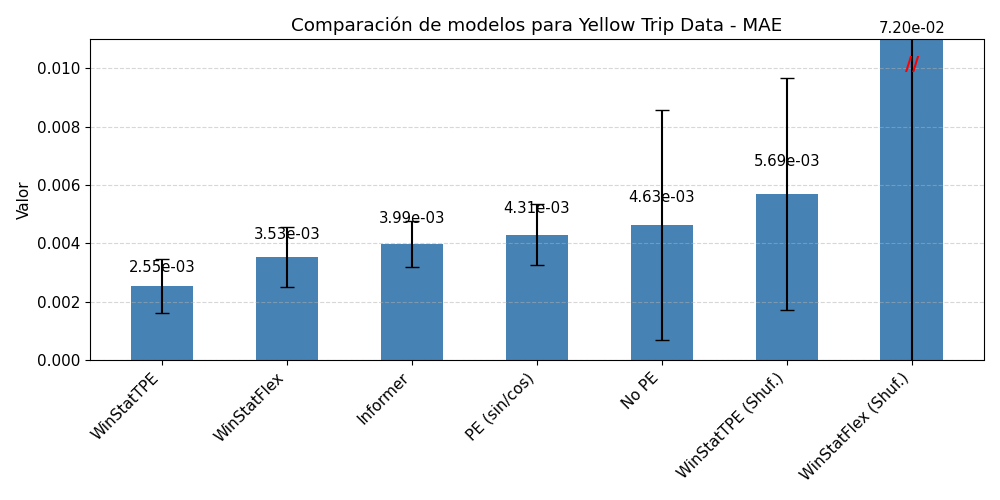
\includegraphics[scale=0.475]{img/taxifinalmae}
	\caption{Yellow Trip data: comparativa gráfica de MAE para los PE evaluados}
	\label{taxifinalmae}
\end{figure}

\begin{figure}[!ht]
	\centering
	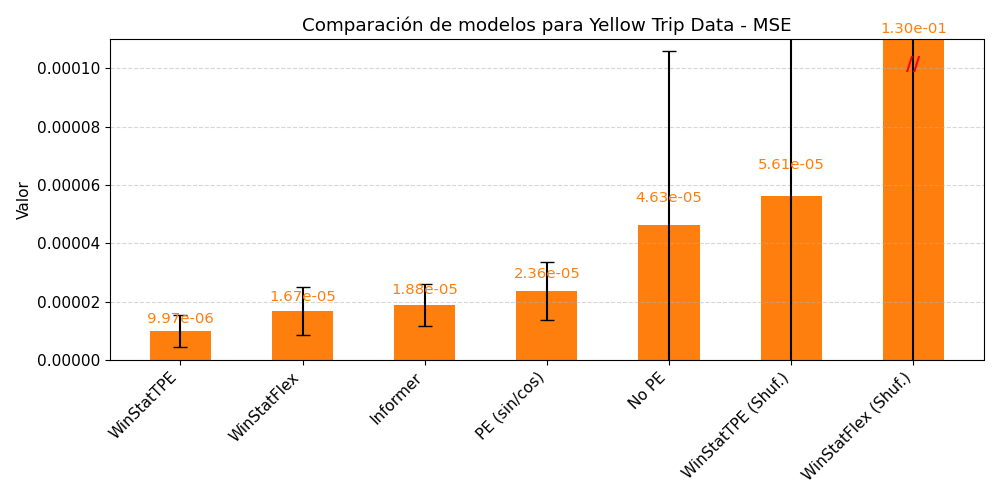
\includegraphics[scale=0.475]{img/taxifinalmse}
	\caption{Yellow Trip data: comparativa gráfica de MSE para los PE evaluados}
	\label{taxifinalmse}
\end{figure}

Podemos apreciar que, en ambos casos, se obtiene el mismo orden entre los algoritmos, por lo que nuestro principal temor de que MSE no fuera representativo, se ha disipado. Contrastado con MAE, las diferencias entre todos los encoding es notable, siendo especialmente notaria la de WinStatTPE, tanto en media como en varianza. Para contrastar los resultados obtenidos para los dos métodos WinStat, se han añadido también las ejecuciones correspondientes al barajado de la entrada del decoder, con el objetivo de medir cuantitativamente el impacto del desordenado en casos donde se codifica una alta localidad. Los resultados se disparan considerablemente, siendo mucho peores que no usar codificación, e incluso sobresaliendo de la gráfica en el caso de WinStatFlex. Esto refuerza de nuevo la gran utilidad de la componente semántica, que no solo mejora los resultados, sino que realmente añade información necesaria a los datos la cual destruye los resultados si es alterada.\\

En resumen, WinStatTPE se puede establecer como el mejor modelo para Yellow Trip data, y su variante Flex supone una buena alternativa. En ambos casos, se añade información fuertemente vinculada al orden y semántica de los datos, que permite mejorar los resultados obtenidos en la predicción, aunque con un mayor coste computacional.


\subsection{TINA: Evaluación de PE}

Como último conjunto de datos disponemos de TINA. Este dataset representa un auténtico reto en términos de complejidad y eficiencia de los algoritmos que se evaluarán a continuación, dado que su elevada dimensionalidad, superior a 103 características por timestamp, exige una gestión cuidadosa de los recursos. Incluso con una optimización profunda, su procesamiento ha demandado una gran potencia de hardware y varios días de tiempo de ejecución. Pero, a pesar las dificultades asociadas, su gran tamaño lo convierte en un benchmark excelente para nuestro método basado en estadísticos y ventanas, tanto a nivel de eficiencia como en efectividad en métricas con respecto a otros modelos del estado del arte.\\

Es importante recordar que este conjunto de datos proviene del ámbito de la detección de anomalías. Por tanto, su objetivo fundamental es evaluar la capacidad de los modelos no solo para predecir la evolución temporal de la serie, sino también para identificar y anticipar comportamientos atípicos. Nuestro problema es principalmente forecasting, por lo que estos puntos anómalos puede ser un complejo reto de solventar, ya que su presencia puede afectar gravemente a las métricas de error y a como se comportan.\\

Este aspecto va referido principalmente al MSE, nuestra principal métrica de referencia. Debido a que eleva al cuadrado las diferencias entre el valor real y el predicho, tiende a amplificar los errores puntuales generados por dichas anomalías, provocando una sobreestimación del error global y, en consecuencia, inestabilidad en la evaluación del modelo. Por el contrario, MAE, que ha sido nuestra segunda opción hasta ahora, al basarse en la magnitud absoluta de las diferencias sin ponderarlas cuadráticamente, proporciona una medida posiblemente más robusta y representativa en este tipo de contextos.\\

A la hora de analizar los experimentos, debemos de tener este aspecto claro, y contrastar adecuadamente entre ambos valores.

\subsubsection{Análisis y resultados}

A continuación, se mostrarán los resultados de los modelos evaluados, siendo de nuevo los 5 modelos ya valorados Yellow Trip y ETTh. En este caso, los parámetros base empleado para todos ellos han sufrido algunas modificaciones considerables para adquirir mayor información de contexto, ya que este dataset tiene un intervalo de medición de 30 segundos. En la tabla \ref{ajustestina}, podemos ver los valores, donde destaca especialmente la longitud de secuencia de 288. Sin embargo, la ventana empleada es de 60, indicando que tomamos únicamente la última media hora. Esto se debe a que aumentar el tamaño hasta alcanzar la heurística comentada en HPC de 1/3 o 1/4 de la longitud de secuencia generaba problemas de reserva de memoria.

\begin{table}[!ht]
	\centering
	\begin{tabular}{l|l}
		\toprule
		Parámetro & Valor \\
		\midrule
		{Modelo de atención} & Vanilla \\
		{Tamaño de batch} & 32 \\
		{Dropout} & 0.2 \\
		{Nº de ejecuciones} & 3 \\
		{Tamaño de ventana} & 60 \\
		{Longitud de secuencia} & 288 \\
		{Longitud de etiqueta/contexto} & 96 \\
		{Longitud de predicción} & 48 \\
		\bottomrule
	\end{tabular}
	\caption{TINA: configuración de parámetros comunes empleada para los experimentos}
	\label{ajustestina}
\end{table}

\paragraph{Informer}

Para disponer de una base de comparación, comenzaremos por el análisis de Informer. En la tabla \ref{tinainformer}, se recopilan los resultados obtenidos por estas métricas. Podemos ver que el valora del MSE es bastante alto en comparación con el obtenido para MAE, como ya anunciábamos en la introducción. Además, el resto de métricas también han subido considerablemente, debido al gran impacto de los errores, potencialmente en los puntos de anomalía, que disparan su penalización.\\

 Los tiempos de ejecución, de manera sorprendente, no han aumentado de forma significativa, manteniéndose entre los valores obtenidos con Household Power o Yellow Trip Data. Esto sugiere que las operaciones asociadas al encoding se están paralelizando de manera adecuada y, en consecuencia, no representan un coste computacional prohibitivo para el modelo. Sin embargo, este aspecto ha de vigilarse de cerca en las codificaciones ponderadas, donde el impacto podrá ser mayor.

\begin{table}[!ht]
	\centering
	\begin{tabular}{l|N|N}
		\toprule
		\text{Métrica} & \text{Media} & \text{STD} \\
		\midrule
		MSE & 1,096588 & 0,106495 \\
		MAE & 0,356679 & 0,020001 \\
		MAPE & 2,780652 & 0,213355 \\
		MSPE & 110744,161458 & 41945,4380 \\
		RMSE & 1,045978 & 0,050186 \\
		TrainTime(s) & 6437,735532 & 1826,084507 \\
		TestTime(s) & 75,916715 & 1,479102 \\
		\bottomrule
	\end{tabular}
	\caption{TINA: métricas de rendimiento para Informer}
	\label{tinainformer}
\end{table}

\paragraph{PE sinusoidal}

Con el fin de evaluar si el modelo Informer, utilizando su esquema de codificación por defecto, ofrece un rendimiento superior al diseño original de los Transformers, analizaremos a continuación los resultados obtenidos al aplicar exclusivamente la codificación seno–coseno a los datos.\\

En la tabla \ref{tinasincos} se muestran los resultados obtenidos para todas las métricas. De nuevo, tenemos que descartar las métricas diferentes a MAE y MSE, que por desgracia, se ven demasiado afectadas por los efectos de las anomalías y aumentan desproporcionadamente su valor. Pero, si nos fijamos en las dos escogidas, podemos ver que se produce un empeoramiento considerable del resultado, especialmente en MSE, debido al efecto potenciador del cuadrado. En MAE también es apreciable, aunque de forma más suave, suponiendo un empeoramiento de $0,03$ sobre Informer. El tiempo de ejecución también ha aumentado, debido a que la convergencia ha sido más lenta y se ha requerido un mayor número de épocas, y no compensa que el coste de la codificación sea menor.

\begin{table}[!ht]
	\centering
	\begin{tabular}{l|N|N}
		\toprule
		\text{Métrica} & \text{Media} & \text{STD} \\
		\midrule
		MSE & 1,247064 & 0,137599 \\
		MAE & 0,386111 & 0,016464 \\
		MAPE & 3,130485 & 0,223893 \\
		MSPE & 83611,562500 & 5558,4220 \\
		RMSE & 1,115078 & 0,060539 \\
		TrainTime(s) & 10709,456470 & 3030,954371 \\
		TestTime(s) & 191,650185 & 0,539033 \\
		\bottomrule
	\end{tabular}
	\caption{TINA: métricas de rendimiento para encoding seno-coseno}
	\label{tinasincos}
\end{table}

\paragraph{WinStatFlex}

Para WinStatFlex, podemos encontrar los resultados para las métricas en la tabla \ref{tinaflex}, mientras que los pesos de la suma ponderada se ubican en la tabla \ref{tinaflexpesos}.

\begin{itemize}
	\item El rendimiento del modelo requiere un análisis cuidadoso de las métricas. Si tomamos como referencia el MSE, su valor, $1,148$, nos hace entender que este modelo es considerablemente peor a Informer, que arrojaba $1,0965$. Sin embargo, si nos fijamos en el MAE, que por definición es más estable para este problema, apreciamos una mejora, pues pasamos del $0,3566$ de Informer a $0,317$, siendo una mejora de 0,038 aproximadamente (11,9\%). Teniendo en cuenta la suposición realizada sobre MAE, estableceremos que el rendimiento de este modelo es, por tanto, positivo.
	
	\item Los pesos del modelo (tabla \ref{tinaflexpesos}) arrojan resultados relevantes de comentar. La componente asociada a estadísticos y lags parece ser la más relevante de todas, siendo el 38,14\% de la ponderación. La codificación fija es el encoding absoluto que más predomina de los 3, alcanzando una aportación del 27,52\%. Las variantes LPE, pero especialmente tAPE, cobran un menor protagonismo en los resultados.
	
	\item Por último, el tiempo promedio de entrenamiento ha aumentado hasta las 7 horas, siendo muy más alto que el visto en Informer, concretamente 4 veces más. Observando la escasa distancia entre modelos, Informer ofrece un resultado más equilibrado tiempo-resultados, indicando a priori, a falta de confirmar en TPE, que en series de mayor extensión el impacto de la semántica ayuda, pero el sobrecoste a pagar puede ser demasiado elevado.
\end{itemize}
 
\begin{table}[!ht]
	\centering
	\begin{tabular}{l|N|N}
		\toprule
		\text{Métrica} & \text{Media} & \text{STD} \\
		\midrule
		MSE & 1,148123 & 0,101258 \\
		MAE & 0,317082 & 0,007091 \\
		MAPE & 2,523967 & 0,158450 \\
		MSPE & 48155,902018 & 22603,7360 \\
		RMSE & 1,070447 & 0,047603 \\
		TrainTime(s) & 25612,583748 & 2671,774248 \\
		TestTime(s) & 471,924614 & 4,538266 \\
		\bottomrule
	\end{tabular}
	\caption{TINA: métricas de rendimiento para WinStatFlex}
	\label{tinaflex}
\end{table}
 
\begin{table}[!ht]
	\centering
		\begin{tabular}{l|N}
		\toprule
		Componente & \text{Peso aprendido} \\
		\midrule
		Stats & 0,3814 \\
		PE & 0,2752 \\
		LPE & 0,1918 \\
		tAPE & 0,1515 \\
		\bottomrule
	\end{tabular}
	\caption{TINA: valores aprendidos en los pesos del encoding WinStatFlex}
	\label{tinaflexpesos}
\end{table}

\paragraph{WinStatTPE}

El siguiente encoding evaluado es WinStatTPE, cuyas métricas podemos encontrar en la tabla \ref{tinatpe} y los pesos correspondientes a las componentes en la tabla \ref{tinatpepesos}. Podemos destacar los siguientes aspectos:

\begin{itemize}
	\item Las métricas de rendimiento siguen el mismo comportamiento que el visto en WinStatFlex: MSE muestra un empeoramiento respecto a Informer, pero MAE establece que se ha producido una mejora, pero tanto con Informer como con WinStatFlex. Por tanto, siguiendo nuestro razonamiento sobre la estabilidad de las métricas, y atendiendo únicamente a MAE, estamos consiguiendo una mejora de $44^{-3}$ con respecto a Flex, pero una considerablemente mayor con Informer, ya que hemos pasado de $0,356679$ a $0,317082$.
	
	\item La distribución de pesos ha cambiado significativamente, optando ahora por una configuración mucho más equilibradas en todas las componentes. Tan solo destacar que las de mayor relevancia, por poco margen, parecen ser TPE y los valores estadísticos, ambas con el mismo peso normalizado de $0,263$.
	
	\item Por último, el rendimiento sigue siendo un aspecto crítico, requiriendo ahora un promedio de 10 horas para completar el entrenamiento. Al menos, la varianza de este parece menor, ya que en todos los casos el modelo ha requerido 6 épocas antes de detenerse por early stopping.
\end{itemize}


\begin{table}[!ht]
	\centering
	\begin{tabular}{l|N|N}
		\toprule
		\text{Métrica} & \text{Media} & \text{STD} \\
		\midrule
		MSE & 1,133453 & 0,121601 \\
		MAE & 0,312652 & 0,021571 \\
		MAPE & 2,544894 & 0,114816 \\
		MSPE & 49108,398700 & 23029,2045 \\
		RMSE & 1,063045 & 0,058214 \\
		TrainTime(s) & 35866,691845 & 116,147264 \\
		TestTime(s) & 438,925862 & 12,634359 \\
		\bottomrule
	\end{tabular}
	\caption{TINA: métricas de rendimiento para WinStatTPE}
	\label{tinatpe}
\end{table}

\begin{table}[!ht]
	\centering
	\begin{tabular}{l|N}
		\toprule
		Componente & \text{Peso aprendido} \\
		\midrule
		Stats & 0,263 \\
		PE & 0,245 \\
		LPE & 0,229 \\
		TPE & 0,263 \\
		\bottomrule
	\end{tabular}
	\caption{TINA: valores aprendidos en los pesos del encoding WinStatTPE}
	\label{tinatpepesos}
\end{table}

En definitiva, parece que este modelo es capaz de ofrecer mejor rendimiento que Informer y WinStatFlex, pero asumiendo un coste aún mayor con respecto a ambos en tiempo de ejecución. Dicho incremento podría incluso llevarnos a decantarnos por la variante Flex, debido a la escasa diferencia promedio encontrada en MAE, en caso de que necesitásemos implementar un sistema real de predicción con estos datos.

\paragraph{Informer sin PE}

Por último se ha ejecutado un modelo sin ningún tipo de codificación posicional para medir el impacto de su ausencia. Tal y como se muestra en la tabla \ref{tinanope}, su rendimiento en cuanto MAE es el segundo peor de todos los modelos evaluados, evidenciando la necesidad de encoding. Curiosamente, la codificación seno-coseno sí que se encuentra clasificada por detrás, obteniendo aún peores resultados, emulando una situación muy similar a la ya vista con ETTh2. Al igual que en este último, es probable que la ausencia de contenido semántico en la codificación posicional tradicional no permita un correcto ordenamiento de la información al no apoyarse en la relatividad y la semática y los resultados se vean alterados negativamente.

\begin{table}[!ht]
	\centering
	\begin{tabular}{l|N|N}
		\toprule
		Métrica & \text{Media} & \text{STD} \\
		\midrule
		MSE & 1,225175 & 0,213712 \\
		MAE & 0,366518 & 0,017925 \\
		MAPE & 2,872100 & 0,106873 \\
		MSPE & 74118,093750 & 52512,970000 \\
		RMSE & 1,102336 & 0,100149 \\
		TrainTime(s) & 14390,446017 & 7472,113055 \\
		TestTime(s) & 212,148864 & 0,769808 \\
		\bottomrule
	\end{tabular}
	\caption{TINA: métricas de rendimiento  en ausencia de PE}
	\label{tinanope}
\end{table}


\subsubsection{Eleccióin del mejor modelo}

Ahora que disponemos de todas las métricas recopiladas para cada modelo, podemos proceder a ordenar los resultados y ver las diferencias entre todas las propuestas. Al igual que en los conjuntos anteriores, podemos observar los resultados en la tabla \ref{tinafinal}, donde los modelos han sido ordenados por MSE. Adicionalmente, se han incluido las variantes barajadas de WinStatFlex y WinStatTPE para verificar el comportamiento de los modelos cuando se rompe el orden temporal. Para una comparación más intuitiva, se ha incluido adicionalmente el gráfico de barras \ref{tinafinal1}.

\begin{table}[h!]
	\centering
	\begin{tabular}{l|N|N|N|N}
		\toprule
		Modelo & \text{MSE (Media)} & \text{MSE (STD)} & \text{MAE (Media)} & \text{MAE (STD)} \\
		\midrule
		Informer & 1,0965 & 0,1064 & 0,3566 & 0,0200 \\
		WinStatTPE & 1,1334 & 0,1216 & 0,3126 & 0,0215 \\
		WinStatFlex & 1,1481 & 0,1012 & 0,3170 & 0,0070 \\
		No PE & 1,2251 & 0,2137 & 0,3665 & 0,0179 \\
		PE (sin/cos) & 1,2470 & 0,13759 & 0,3861 & 0,0164 \\
		WinStatFlex (Shuf.) & 1,3399 & 0,1100 & 0,5094	 & 0,1025 \\
		WinStatTPE (Shuf.) & 1,4412 & 0,1025 & 0,4511 & 0,0061 \\
		\bottomrule 
	\end{tabular}
	\caption{TINA: resultados ordenados por MSE, incluyendo modelos barajados}
	\label{tinafinal}
\end{table}

\begin{figure}[!ht]
	\centering
	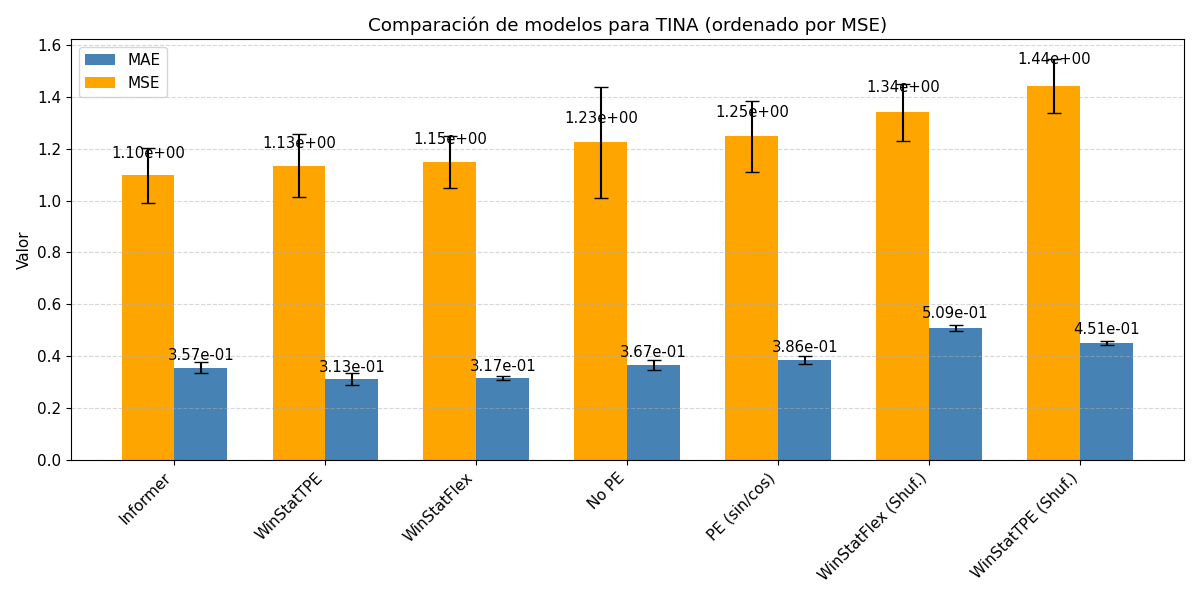
\includegraphics[scale=0.45]{img/tinafinal1}
	\caption{TINA: comparativa gráfica ordenada por MSE para los PE evaluados}
	\label{tinafinal1}
\end{figure}

Se puede apreciar que la distancia entre los tres primeros modelos es muy pequeña. Las variantes TPE y Flex se encuentran muy próximas entre sí, a $0,01$ de diferencia, mientras que Informer parece mostrar un rendimiento más diferenciador si tenemos en cuenta el MSE. Por su parte, desordenar la estructura temporal de la serie en el decoder está rompiendo la naturaleza de la serie y su localidad asociada tanto para WinStatFlex como para WinStatTPE. Pero, si en su lugar miramos el MAE, vemos que la diferencia entre los tres mejores es más alta. Por tanto, aunque pueda parecer que nuestra propuesta no funciona tan bien como en casos anteriores, si lo esta haciendo pero MSE puede distorsionar un poco los resultados por la propia naturaleza de TINA.\\

\begin{figure}[!ht]
	\centering
	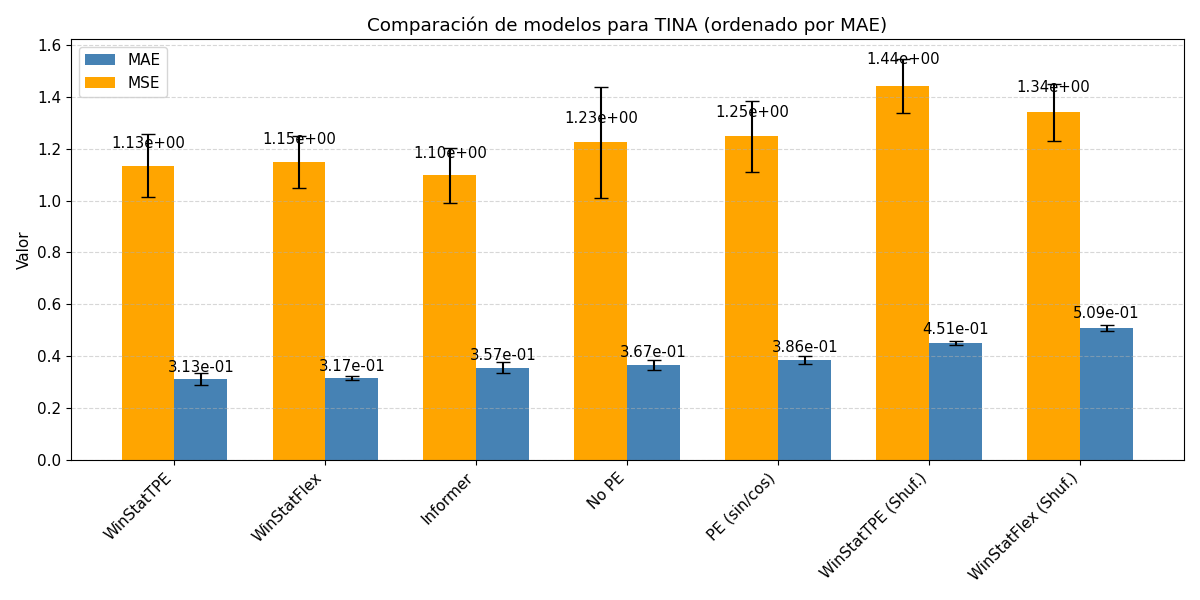
\includegraphics[scale=0.45]{img/tinafinal2}
	\caption{TINA: comparativa gráfica ordenada por MAE para los PE evaluados}
	\label{tinafinal2}
\end{figure}

Ordenando los modelos por MAE, la situación resulta mucho más cercana a todos los casos anteriores. Como se puede apreciar en la figura \ref{tinafinal2}, ahora los modelos barajados pasan al final de la lista, y los encodings WinStatTPE y WinStatFlex ocupan los dos primeros lugares en ese orden, con una escasa diferencia entre sí. Informer queda en tercera posición, seguido de cerca por el modelo no codificado y el de seno-coseno, poniendo así en jaque las propiedades del modelo original. Pero este efecto puede verse potenciado por las escasas diferencias, a nivel general, entre todos los modelos ejecutados, fruto de la extensa longitud y anchura del dataset, que dificulta su codificación.\\

Por tanto, podemos concluir que los modelos WinStatTPE y WinStatFlex son los mejores para este conjunto de datos, siguiendo así la misma tendencia que los 3 anteriores datasets. Sin embargo, es importante destacar que, dada la distancia mínima entre los resultados de TPE y Flex, usar la segunda variante podría ser más razonable en caso de que el tiempo de entrenamiento sea clave, ya que el tiempo requerido para este es, en promedio, menor.

\section{Resumen final}

Con la finalización del análisis y experimentación sobre el dataset TINA, disponemos de los resultados para todos los modelos evaluados, lo que nos permite ver, de manera global, el funcionamiento de cada uno de ellos, y su consistencia en cuanto a resultados sobre el resto de modelos. En la tabla \ref{resumenfinal}, se puede encontrar en formato apaisado los valores obtenidos tanto para MAE como para MSE, destacando en negrita los mejores resultados, para así distinguir fácilmente el mejor modelo en cada dataset. A modo de síntesis, de manera general podemos extraer las siguientes conclusiones:

\begin{itemize}
	\item Aunque no estén explícitamente ejecutados, los modelos WinStat y más concretamente, WinStatLag, han sido la base de este experimento. Podemos ver que en todos los datasets, el modelo con mejor rendimiento era uno de los que empleaba WinStatLag como primera componente aditiva del producto ponderado, demostrando que este concepto ha permitido capturar una mayor información local y contextual del problema, permitiendo reducir al falta de semántica que tanto caracterizan a los encodings tradicionales geométricos. 
	
	Sin embargo, a pesar de ser una componente decisiva, ésta no ha funcionado correctamente cuando se emparejaba con SPE. Esto se debe, tal y como describimos en su definición, que los mecanismos de atención modificados pueden llegar a dificultar el rendimiento de los modelos de forecasting, aunque permite reforzar la identificación de segmentos temporales muy concretos para clasificación. Pero esto no era contexto de nuestro análisis, más orientado a forecasting, por lo que su uso estaba fuera de lugar.
	
	 Para verificar que no se trataba de un efecto de complementariedad con WinStatLags, se evaluó de manera independiente utilizando Informer original, a modo de ablation study. Sin embargo, como se observó en el conjunto HPC, los resultados seguían siendo significativamente inferiores a los obtenidos por las demás variantes, lo que motivó su descarte en los siguientes conjuntos de datos. Esto deja a WinStatLags como pieza clave del rendimiento, gracias a sus estadísticos y diferencias con rezagos.
	 
	 \item La ponderación de componentes aditivas ha permitido mejorar considerablemente el rendimiento del modelo sin parámetros extra. Gracias a emplear pesos entrenables, la combinación aditiva de encodings vista en WinStatFlex y WinStatTPE ha permitido obtener mejoras considerables de rendimiento respecto a nuestro algoritmo de referencia, sin necesidad de requerir al usuario su especificación. De esta forma, mediante la función de pérdida, podemos ir ajustando para obtener siempre los mejores resultados, llegando incluso a anular componentes si fuera necesario. El único aspecto a tener en cuenta es que debemos ser cuidadosos con su inicialización y rango, pero empleando Softmax podemos controlarlos sin problemas.
	 
	 \item El dominio de WinStatFlex es bastante marcado. Aunque en numerosas ocasiones, como TINA y Yellow Trip, la variante TPE ha conseguido prácticamente igualar o superar su rendimiento, en promedio, WinStatFlex ha sido capaz de agregar eficazmente información posicional al modelo, mejorando considerablemente los resultados y diferenciándose claramente de Informer. Aunque su eficiencia temporal es mucho mayor a este, el diferencia de rendimiento es lo suficientemente significativo como para ser una alternativa justificable sobre la definición tradicional.
	 
	 \item WinStatTPE resulta una alternativa interesante para WinStatFlex, pero se ve lastrado por su rendimiento. Los resultados generados por este encoding son también atractivos, dejándolo en segunda posición en cuanto a lo que rendimiento respecta. Su baja varianza en los resultados indica que se trata de un algoritmo muy estable numéricamente y que suele converger en puntos similares en sucesivas ejecuciones. Sin embargo, su tiempo de ejecución es considerablemente más elevado, por lo que en problemas donde la estabilidad numérica es crítica, como vimos en Yellow Trip o TINA, su rendimiento destaca, pero por lo general, se recomendaría el uso de WinStatFlex.
\end{itemize}

Por tanto, tal y como se puede apreciar en la tabla \ref{resumenfinal}, siguiendo la metodología aplicada en el paper de Informer\cite{zhou2021informerefficienttransformerlong} y realizando el recuento de ejecuciones en primer lugar, obtenemos el siguiente orden por rendimiento:

\begin{enumerate}
	\item \textit{WinStatFlex}
	\item \textit{WinStatTPE}
	\item \textit{Informer}
	\item \textit{PE geométrico (seno-coseno)}
	\item \textit{Sin uso de PE (No PE)}
\end{enumerate}

\clearpage
\begin{landscape}
	\vspace*{\fill} % empuja el contenido hacia el centro vertical
	\begin{table}[H]
		\centering
		\huge
		\resizebox{\linewidth}{!}{%
			\setlength{\tabcolsep}{7pt}%
			\renewcommand{\arraystretch}{2}%
			\begin{tabular}{c|cc|cc|cc|cc|cc}
				\toprule
				\multirow{2}{*}{\begin{tabular}{c}Modelo \\ Métrica\end{tabular}} 
				& \multicolumn{2}{c|}{Informer} 
				& \multicolumn{2}{c|}{PE (sin/cos)} 
				& \multicolumn{2}{c|}{WinStatFlex} 
				& \multicolumn{2}{c|}{WinStatTPE} 
				& \multicolumn{2}{c}{No PE} \\
				\cmidrule(lr){2-3}\cmidrule(lr){4-5}\cmidrule(lr){6-7}\cmidrule(lr){8-9}\cmidrule(lr){10-11}
				& MSE & MAE & MSE & MAE & MSE & MAE & MSE & MAE & MSE & MAE \\
				\midrule
				HPC         & $0,5329$ & $0,4152$ & $0,5377$ & $0,4140$ & $\mathbf{0,4618}$ & $\mathbf{0,3734}$ & $0,4636$ & $0,3743$ & $0,5448$ & $0,4213$ \\
				\addlinespace
				ETTh1       & $0,5458$ & $0,5324$ & $0,5776$ & $0,5552$ & $\mathbf{0,4660}$ &$\mathbf{0,4947}$ & $0,4896$ & $0,5072$ & $0,9235$ & $0,7419$ \\
				\addlinespace
				ETTh2       & $0,8866$ & $0,7549$ & $1,3881$ & $0,9355$ & $\mathbf{0,4677}$ & $\mathbf{0,5128}$ & $0,5964$ & $0,5889$ & $1,0132$ & $0,7777$ \\
				\addlinespace
				Yellow Trip & $1,9 \times 10^{-5}$ & $3,987 \times 10^{-3}$ & $2,4 \times 10^{-5}$ & $4,307 \times 10^{-3}$ & $1,7 \times 10^{-5}$ & $3,529 \times 10^{-3}$ & $\mathbf{1,0 \times 10^{-5}}$ & $\mathbf{2,547 \times 10^{-3}}$ & $4,6 \times 10^{-5}$ & $4,626 \times 10^{-3}$ \\
				\addlinespace
				TINA        & $\mathbf{1,0965}$ & $0,3566$ & $1,2470$ & $0,3861$ & $1,1481$ & $0,3170$ & $1,1334$ & $\mathbf{0,3126}$ & $1,2251$ & $0,3665$ \\
				\addlinespace
				\midrule
				\midrule
				Count & \multicolumn{2}{c|}{1} & \multicolumn{2}{c|}{0} & \multicolumn{2}{c|}{\textbf{6}} & \multicolumn{2}{c|}{3} & \multicolumn{2}{c}{0} \\
				\bottomrule
			\end{tabular}%
		}
		\caption{Resumen final: resultados para MAE y MSE en cada dataset}
		\label{resumenfinal}
	\end{table}
	\vspace*{\fill} % completa la parte inferior para centrar verticalmente
\end{landscape}
\clearpage








